\documentclass[a4paper,12pt]{report}
\usepackage[hmargin=1in, vmargin=1in]{geometry}
\usepackage[shortlabels,inline]{enumitem}
\usepackage[labelfont=bf]{caption}
\usepackage{xcolor, amsmath, amssymb, array, booktabs, multicol, multirow, setspace, hyperref, graphicx, rotating, pgf, hyperref}

\hypersetup{
    colorlinks,
    citecolor=black,
    filecolor=black,
    linkcolor=black,
    urlcolor=blacks
}

\newcommand{\link}[2]{\hyperlink{#1}{\underline{#2}}}
\newcommand{\msection}[1]{\noindent\textbf{#1}}
% \doublespacing
\newcommand{\authorname}[3]{
    \begin{minipage}[t]{.25\linewidth}
        \centering
        \textbf{#1} \\
        \small #2 \\
        #3
    \end{minipage}
}

\newenvironment{bottom}{\par\vspace*{\fill}}{\clearpage}

\begin{document}

\begin{titlepage}
    \centering
    \Large\textbf{Group 20: Everglades Analytics Design Document}
    \normalsize
    \vspace*{.25in}
    
    % First name alphabetical order 
    % Elaine Ng, Ian Pleau, Manuel Vasquez, Ossama Amer, Thomas Lukas
    
    \authorname{Elaine Ng}{Computer Science (BS)}{Statistics (BS)}
    \authorname{Ian Pleau}{Computer Science (BS)}{}
    \authorname{Manuel Vasquez}{Computer Science (BS)}{Statistics Minor}
    \vspace*{.125in}
    
    \authorname{Ossama Amer}{Computer Science (BS)}{}
    \authorname{Thomas Lukas}{Computer Science (BS)}{SCAN Minor}
    
    \vspace*{.25in}
    \today
    
    \vspace*{.4in}
    \noindent\rule{.5\linewidth}{.4pt}
    \vspace*{.4in}

    % flushes logos to bottom
    % \begin{bottom}
        \begin{minipage}[c]{.35\linewidth}
            \centering
            
\includegraphics[width=1\linewidth]{media/lm.png}
        \end{minipage}
        \begin{minipage}[c]{.3\linewidth}
            \centering
            
\includegraphics[width=.2\linewidth]{media/ucf.png}
        \end{minipage}
    % \end{bottom}
\end{titlepage}

\onehalfspacing
\pagenumbering{roman}

\tableofcontents

\newpage

\setlength{\parskip}{\baselineskip}
\setlength{\parindent}{0in}
\pagenumbering{arabic}

\chapter{Executive Summary}
\section{Goals and Objectives}
\subsection{Goal \#1}

\textit{Characterize StarCraft match output from a publicly available dataset to determine behaviors that most often lead to wins.}

\textbf{Description |} StarCraft match output data sets would be analyzed to identify characteristics. Characteristics that are statistically significant in determining the win rate would be clearly documented and be used for the other goals in predicting match outcomes. Characteristics that are not statistically significant in determining win rate will not be considered for behaviors that most often lead to wins but will still be recorded for the reason that it might help increase the accuracy of match outcome prediction.

\textbf{Specifications |} We suggest that for this goal we should find at least 5 characteristics that are statistically significant in determining the win rate. Optimistically, we would be able to identify more winning behaviors, as well as filter out the statistically insignificant characteristics that we might have identified during the process. 

\subsection{Goal \#2}

\textit{Propose new metrics to predict agent performance, similar to Sabermetrics.}

\textbf{Description |} Research should be done on StarCraft and data sets should be analyzed in order to find new metrics that are statistically significant in predicting agent performance and their match outcomes. Such as, but not limited to, action per minute (APM), damage per second (DPS), strategies used, micro and macro.

\textbf{Specifications |} We suggest that for this goal we should find at least 5 new metrics that are statistically significant in predicting agent performance. Optimistically, we would be able to propose more metrics that can be utilized to predict agent performance. We hope that with these newly proposed metrics, we are able to predict outcomes more accurately and demonstrate the reasons behind agents’ match outcomes. 

\subsection{Goal \#3}

\textit{Identify how map differences affect the output of games with similar strategies.}

\textbf{Description |} Research should be done on StarCraft maps and the types of strategies. The differences between maps and the types of strategies available on StarCraft should be identified. The map differences that are statistically significant in affecting game outputs with similar strategies will be clearly documented.

\textbf{Specifications |} We suggest that for this goal we should find at least 3 map characteristics that are statistically significant in affecting the output of games with similar strategies. Optimistically, we would be able to find more map differences that have an effect on game output and be able to show which strategy works best for the different types of maps.

\subsection{Goal \#4}

\textit{Implement a supervised machine learning classification algorithm that predicts the outcome of a match given the current game state.}

\textbf{Description |} We would build a software analysis tool that can take in the specific details of the match and correctly have a successful prediction of future game results. Using the previous must-have requirements, the algorithm should be able to use those metrics to accurately predict which player is expected to come out victorious.

\textbf{Specifications |} We suggest that this algorithm should have above a 75\% accuracy when predicting after the early game, early game predictions in StarCraft can easily fluctuate based on human player blunders and strategy implementation. The stretch end goal is to produce an algorithm that can predict with high accuracy at any point in the match.

\subsection{Goal \#5}

\textit{Develop a real-time analytics engine that runs simultaneously with StarCraft match playback. The engine should be at a minimum to predict odds of winning and describe the agent behaviors.}

\textbf{Description |} The home run goal of the entire project is to create a real-time predictor, similar to something you would see in a poker match on TV. In those poker games, the hand odds are calculated and predicted win probabilities are given to each player competing in the current hand shown in real-time. Similarly, the software program we would develop would take in the metrics provided in the goals above and output a real-time predicted win probability every five seconds or so.

\textbf{Specifications |} We suggest that this algorithm should have a plausible enough accuracy at every point of the game. Similar to the stretch goal above, after the early game the algorithm should have above a 75\% accuracy of predicting the correct outcome. Starting from early game strategies and economies, the predictor should never give a player a near 100\% accuracy to win right before they blunder and lose the game. Although human error may always provide outliers, this should not be an excuse for the predictor on average to have a below-average prediction accuracy.  

\section{Personal Motivations}

\msection{Elaine Ng}

When I first heard the Everglades’ project pitch, I was immediately interested because it was a strategy video game. Then the different teams for the project were presented and I saw that there was going to be an Analytics Team. I knew at that moment that the Everglades: Robot Behavior Analytics Team was the perfect senior design project for me. As someone who spends a lot of time playing video games and is also currently studying for a Computer Science and Statistics degree, I felt that this project brought many of my passions together. Having the opportunity to learn how to gather, analyze, and predict for large video game data sets with a dedicated team and knowledgeable guidance is definitely one of my main motivations for the Everglades project. This will be one of my largest projects yet, and I am very excited to be a part of this.

\msection{Ian Pleau}

The everglades projects were presented by Lockheed all in one go and immediately they all ranked highly on my list of preferred projects. The idea of working on a real-time strategy(RTS) type project and having the opportunity to either work on the game side of the database and analytics side piqued my interest. Ultimately, I leaned more towards the analytics side choosing that as my first choice. My reasoning for this choice was that I always in the past had been heavily focused on numbers and data when looking to optimize in games, programming, or even just decisions I would make in day to day life. The project was initially proposed with the possibility of working with Everglades data but also working with StarCraft data to create a baseline idea for how to analyze a win rate and a real-time strategy data set.

\msection{Manuel Vasquez}

I think I’m in the wrong major. When I began university I just wanted to learn how to code, but as I progressed through my courses I realized that I’m actually more interested in gathering insights from otherwise obscure data. This project is giving me the opportunity to acquire real-life skills and learn how to present my findings to professionals in other fields. The club AI@UCF introduced me to the basics of many libraries like Tensorflow, Torch, and Sci-kit learn. UCF taught how to find statistically relevant information from simple datasets. Now I’m able to merge these two knowledge bases into what we’re calling Everglades Analytics.

I’ve attended enough lectures about reinforcement learning to know that I have no idea what I’m doing. Thankfully, this project focuses on the analytics aspect of the Everglades project. Novel models like AlphaStar have greatly advanced the area of reinforcement learning. With many research papers discussing the developers’ ground-breaking approaches and the model’s super-human performance on several real-time strategy games. Given AlphaStar’s almost perfect approach to Starcraft, we can study this model and possibly discover actionably better strategies than our current STARDATA dataset can provide.

\msection{Ossama Amer}

Due to my interest in Data Science, I was ecstatic to participate in this project. Acquiring analytics from a real-time military science game in order to match output to attain the most wins is something I feel I can greatly benefit from as a computer science student. We look forward to making our sponsors proud and more importantly, delivering efficient results, further bettering the EVERGLADES project through artificial intelligence advancement. Aside from the project, I also look forward to networking with my teammates and developing new connections while discovering new technologies.

\msection{Thomas Lukas}

When the initial project was presented, I was immediately hooked with the idea of a strategy game that can be used as a foundation to teach the process of creating and training AI. Strategy board games and video games have always been a big part of my life growing up, I always tried my hardest to discover and sometimes attempt to create a new "meta" that can balance the odds in my favor. Working with StarCraft data, I am more than excited to see the mathematical representation that each "meta" strategy implemented by the factions will look like in the grand scheme of things. I am eagerly looking forward to getting the results and seeing what strategies could be potentially translated to the EVERGLADES project for future teams in senior design around the nation.

\section{Broader Impacts}

For an immediate impact of the project working with a popular game like StarCraft 2 can make the project applicable to a wide player base to use it as a way of improvement. More importantly for EVERGLADES due to the similarity of EVERGLADES and StarCraft 2 the analysis and tools developed on this project could become relevant to Everglades. This is supported by the impact of StarCraft 2 being a much more complex game so if a porting were to happen it would generally be simplifying the work already done. With this ported analysis and tools it could potentially be used by future Everglades teams and workers in order to fine tune balance and design for the future.

The "broader impact" of this project is to set up a baseline for further research into successful strategies for RTS games, specifically applying this to the everglades project. With the Everglades project acting as an RTS training simulator for the strategy of drones, the information and statistics of the unit management and efficiency could become a stepping stone for further research and real-life application. Talking specifically about Lockheed as a military contractor data analysis of drone strategies could eventually lead to enhancements in defense combat or national security and then broader a look into how to manage a fleet of drones efficiently for non-combat uses. Non-combat drone usage could be wide from non-profit work and environmental work to enhanced infrastructure and improvements to the way companies view shipping.

\section{Legal, Ethical, and Privacy Issues}

Legally the work within Data analysis for StarCraft and Everglades is not under NDA. This however does not mean the project is open source and information regarding the sharing and distribution of the programs and analysis that is produced is decided by the sponsor Lockheed Martin. Ethically because we are working with StarCraft data it is hard to say that anything is questionable and there were no problems encountered within it going forward the use of the analysis could be used for efforts that are not as ethical but as of now it is a non-issue. Privacy Issues have also not been a problem nor are they likely to pop up in future use of the implementation.

\chapter{Technical Content}
\section{Project Overview}

The Everglades Agent Behavior Analytics project is a project with the goal to set the baseline for accurate analysis of RTS (Real-Time Strategy) data that is used to learn and infer better strategies for the future. The origin of the use of this analysis is the Everglades RTS game that Lockheed Martin has developed and is being worked on by another team. Due to the current lack of meaningful data, it was important to focus on a similar RTS to get meaningful data and that is where StarCraft comes in. StarCraft as a game is a very complex real-time strategy game, it features three primary archetypes or races to play as, Zerg, Terran, or Protoss, within these races it has thousands of different strategies and ways to play the game and therefore has received a massive following over its long tenure as a popular game. With its massive popularity comes a large data set that is out there known as StarData through this it is possible to completely analyze over 60,000 games of StarCraft data for use.

Everglades as an RTS game has the goals of having specific unit compositions, strategies, base layouts, and more all features that are present in StarCraft which makes it the perfect Game for effective crossover data. The current overarching goal of the project is to utilize statistics, supervised learning, and unsupervised learning to study Behaviors that Lead to Wins, Losses, and other major events that can occur within the StarCraft game. The starting Objectives will be to use the database of info and start setting up some initial learning patterns given the data to focus on Wins and Losses. As the project progresses smaller objectives such as unit compositions will become an objective with setting up algorithms that make these possible.  The function of gathering all this data is overall to have a good basis for further gathering and development of data. With this starting point once the Everglades project has data that is needing to be analyzed the methodology and tools are already developed and ready to go and only need slight changes to switch from being a StarCraft data set to the everglades data.

\section{Project Requirements and Specifications}

\section{Possible Features}

\msection{Elaine Ng}

We could go into a more statistical direction and use regression analysis to attempt to find the relationships between certain variables/characteristics in regards to winning rate, agent performance, and map differences, and the type of strategy used. Perhaps a logistic regression is a good place to start since we are dealing with a categorical dependent variable (win or lose). We can also try to use machine learning methods to predict performance such as supervised or unsupervised learning.

\msection{Ian Pleau}

Going in a research-based direction could be extremely beneficial for this project. This means reading as many papers to get ideas of how we are going to analyze and structure data from StarCraft as possible before going into the data analysis. Starcraft has a lot of statistics that lead to a win or a loss, the key will be to identify which of these stats are the best possible for us to deep analyze. Shoehorning off of Thomas one of the best statistics that could be looked at is definitely the different races and what they mean for playstyle, game times, and win rates at specified moments of the game. This could open a bigger analysis into studying spikes in win rate over time, does minute 30 of a game have a large win rate spike in a certain race because they are able to achieve a powerful unit at that time or other analysis.

\msection{Manuel Vasquez}

To start off the project we should do exploratory data analysis. To gain a deeper understanding of what simple strategies utilized by players we can perform clustering. Applying K-means can render useful results. To continue with the issue of strategy, we could classify approaches by build order (STARDATA. 2017). This can even provide insight into troop usage and the rate of resources mined. This approach would not tell us which strategy is best, since there are other influential factors that also need to be observed, e.g.: warfare handling and enemy status prediction.

\msection{Ossama Amer}

Expanding on Elaine’s idea of delving into a more statistical direction, I think we should also use correlation analysis to explore the relationships between the behaviors and outcomes. Identifying if data is symmetrical and interchangeable is key to verifying if we are acquiring the expected outcomes. If we can pick up on certain actions and behaviors being correlated with wins or losses, that will allow us to dive deeper into the idea of regression analysis and see exactly what causes those outcomes, that way we can modify algorithms accordingly.

\msection{Thomas Lukas}

Initial building and unit decisions are among the most important parts of the game, especially if one of the races in the match is Zerg. Zerg players tend to be overly aggressive in their unit creation and attack tactics so if the opposing player does not implement the correct counter strategy, the Zerg player will snowball into a victory. We believe that if our algorithm can identify the early strategies of both players it can accurately predict a quick win depending on if a player is getting countered perfectly. One problem that can arise however is that since this will be human vs human matches, there is always the chance for the player with the superior strategy to blunder in execution and lose the game.

\section{Distribution of Work}

\section{Project Block Diagram}
\begin{center}
    \captionsetup{type=figure}
    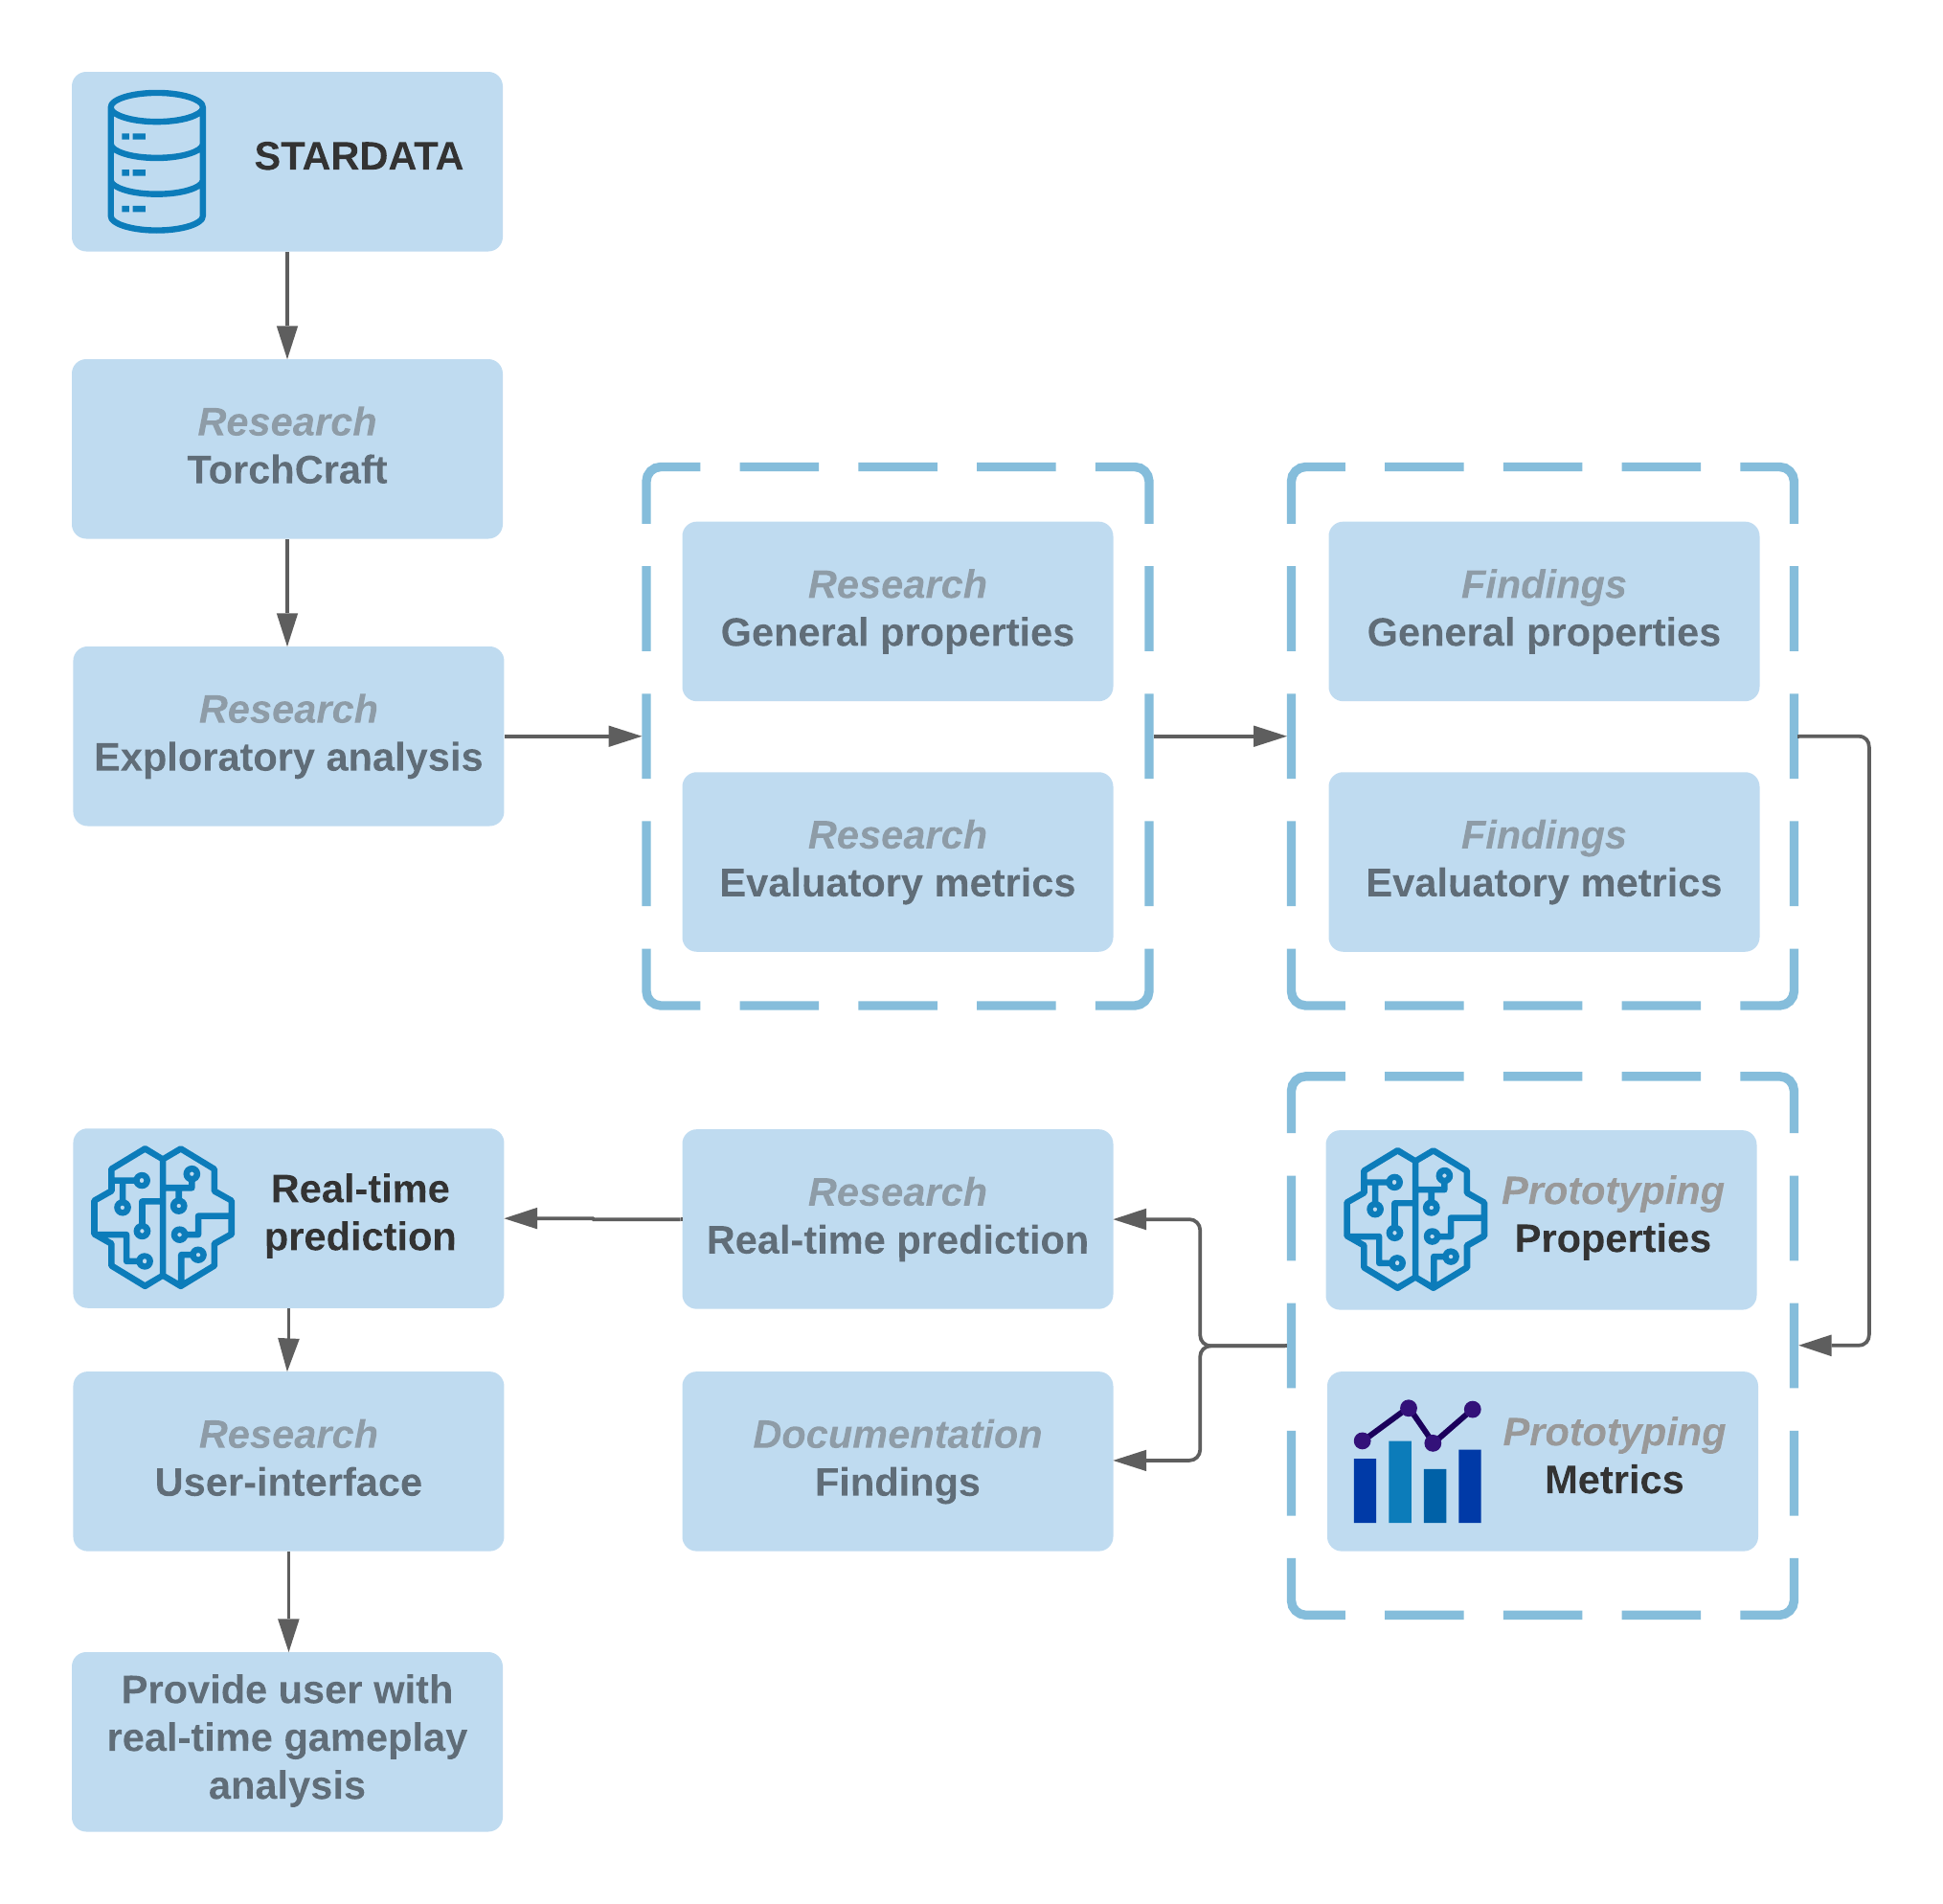
\includegraphics[width=.9\linewidth]{media/block_diagram.png}
    \captionof{figure}{Working project block diagram as of September 30, 2020.}
\end{center}

\section{Milestones}
\subsection{Senior Design I}

\begin{enumerate}
    \item Initial research
    \begin{itemize}
        \item Normalizing machine learning concepts
        \item Reading relevant publications
        \item Acclamation to StarCraft
    \end{itemize}
    \item Dataset and tools exploration
    \begin{itemize}
        \item PySC2, S2Client-Proto3. Statistical analysis
        \item General metrics summary, e.g.: Minerals mined per minute
        \item Map and race clustering
    \end{itemize}
    \item Identify descriptive metrics
    \item Design document
\end{enumerate}

\subsection{Senior Design II}

1. Win prediction engine (WPE) research
- DeepMind set the groundwork for edge cases
2. WPE training and testing feedback loop
3. SC2 overlay UI research
4. Project findings presentation and keynote

\chapter{Research}
\section{Brood War and Torch Craft}

StarCraft Brood War is the initial game proposed by Lockheed Martin for research due to its similarity to the proposed final everglades project. With this proposal Lockheed also brought up the related dataset and API for this game which is Torch Craft. Torch Craft uses Star Data which is a massive dataset of 65000 games to allow deep analysis of frame data within the game. This initial proposal seemed to be the right choice at first but it became apparent pretty quickly that Torch Craft brought with it a unique set of issues. The stem of these issues being mainly the outdated nature of Torch Craft and its surrounding programs.

BW API (Brood Wars API) is the main API Torch Craft pulled from and this API has been without an update for over three years, ordinarily dated software would be fine, but this API uses StarCraft and specifically version 1.16. Recently Blizzard Entertainment the company behind StarCraft remastered the game and with that remastered they updated the game specifically including anti-cheat and anti-bot software with it, in turn this bricked BWAPI from working with the newer version. The initial work around that we located for this was finding an unofficial version of the game that ran on 1.16 and beginning to setup the client and server-side versions of Torch Craft from there. 

Unfortunately, even with the new working version of StarCraft with BWAPI TorchCraft server software was unable to run on Windows versions above Windows 7 and furthermore the linux version seemed to be not working at all in our attempts.

\section{Game Mechanics}

The next logical step after dropping the previous database was finding the correct game to pivot to that had an adequate database and kept the similarities to EVERGLADES that Brood War had initially brought. The obvious choice was to look into the sequel to Brood War, SC2 (StarCraft 2) as it has been a mainstay in the RTS game community and came out within the modern era meaning it was very likely to be able to function on modern architecture and machines. More important even than the game choice was the access to a database and API, luckily for StarCraft 2 it has one of the most robust game API’s and datasets of any modern era game in PySC2 and SC2 API (StarCraft 2 API). The next decision was to bring up the proposed change to Lockheed Martin and they agreed that this was a good choice to make the change and gave the go ahead.

\subsection{Basics}

StarCraft 2 at its core is an RTS or Real Time Strategy game that pits players together on a variety of maps with one goal to destroy the enemies base and force them to concede. Although a simple premise the game becomes very complex very quickly as it layers thousands of strategical choices on top of each other to make one of the most skill and knowledge intensive games out there. At the start of any game each player will be given a choice of race and a map will be chosen when the game starts players will begin with 1 core building and a group of workers which can begin gathering minerals to spend on the task of winning the game.

Minerals and gas are explained in depth in a future section, but they are the core of the games economy and allow for the purchase of the main methods of securing victory which are buildings and units. Buildings usually facilitate the creation of units and improvement of units and require space to place down, units act in various ways generally combat related and build up to be a force used to fight enemies. Combat happens in Real Time and can be dynamic all units and buildings have a set amount of Health Points commonly referred to as HP which when they reach 0 lead to the unit dying or being eliminated.

Controls are simple starting off camera can be moved with arrow keys and units are moved by simply right clicking the location for which you would like them to go. Additionally, units can be selected using left click or drag for multiple units/ double click for all units of a type. These simple controls are very usually switched to more complex controls as players improve though to match the need to be able to easily manage many more units at a single time. Buildings can be selected in the same manner in order to use them, buildings come in varying uses but once selected they can be managed using a variety of hotkeys to research upgrades to units or build units.

\subsection{Races}

Before beginning a game, every player must begin by choosing one of three races between Protoss, Zerg, and Terran each with its own unique set of strengths, weaknesses, and strategies. This choice is where the initial complexity of StarCraft 2 begins, this is because each race shares only the controls of the game with one another, all units, and buildings are race specific and each race has its own niche mechanics that are not shared. Additionally, the following races are not balanced to all be the same average skill level required and some require a large amount more knowledge than others.

\subsubsection{Protoss}

Protoss are a race that generally focus on few units over many they rely on having powerful but expensive units and strong supporting units to make up for the numbers disadvantage they might have. Additionally, Protoss focus on having heavy defense units through their use of shields which give them added health that will regen over time.

Probably the main core feature of the Protoss race is their requirement to power all their buildings with a building called a pylon, this acts as both a blessing and a curse to the Protoss player as it makes it easy for enemies to disable their defenses but it enables their core military feature the warp. Warping is their main military feature and it allows them to spawn in their units nearly instantly and at any position where they have a pylon on the map, this enables creative gameplay and sneak attacks to be extremely powerful as well as creating strategic choices that can quickly lead to victory if not countered properly.

\subsubsection{Zerg}

Zerg could be the opposite of the Protoss; they are strength in numbers, a race that focuses on expanding bases extremely quickly and taking over the map through powerful waves of units. Due to the race having large amounts of units that are weaker but being able to produce them very fast, zerg players generally attack constantly, slowly chipping away at the enemies and forcing them to split their units to deal with the swarm.

Zerg also features a system that has downsides and upsides in their primary method of building, for buildings they must sacrifice one of their collector units in order to build anything this means that they lose income in order to expand but they generally are able to expand faster. Unlike the Protoss warp  zerg builds their units manually out of a unit their bases produce called larvae, due to this being a resource produced by having bases, zerg generally focuses on expanding as quickly as possible. With these seeming downsides of the race comes the upside of being a race that can finish out a game extremely quickly with their most famous strategy named the zerg rush. As seen in the graph below there are huge spikes in game length specifically in all matchups with Z(zerg).

\subsubsection{Terran}

Terran can be viewed as the most well rounded of the three races they are often seen as extremely resourceful and have the ability to pursue similar strategies to the other two races as well as some unique strategies based around their core units and special abilities. Terran have a major strength in their ability to hold a defense line like none of the other races with strong buildings that can be repaired by their builders, additionally they have the ability to dynamically move any of their buildings by lifting them off, this means without strong anti-air units a terran player could potentially stall for a near infinite amount of time.

\subsection{Scouting and Vision}

A core mechanic of StarCraft 2 and similar RTS games is a lack of vision for an area unoccupied by a building or a unit generally referred to as the fog of war. Fog of war is a mechanic that provides the ability for strategy to flourish as it adds another layer of depth to the game. With both players unable to see the opponent from the game start it becomes easy to hide strategies and units that could be massive in upcoming battles this means that it also creates the need to learn what the opponent is doing at all times. Scouting consists of sending units into the fog of war to search for an area that the enemy is using and to discover the strategies and assess the strength of the enemy, although not an immediate tactic to claim victory it is still an important precaution to take to secure victory in the end.

\section{Maps}

In the competitive multiplayer scene, there is a select number of maps that are "in rotation" for players to compete against each other in. Each map elicits different types of strategies and early game builds for each player depending on their chosen race and their opponents’ race.

Online there are tons of guides available for players to see what pros and cons each race has on each of the "in rotation" maps they will be expected to play on in competitive play.

Some important features that affect gameplay in the competitive scene are:

\begin{itemize}
\item The distance between both starting base positions. \\
More space would elicit more of an expansion-based build orders, whereas if there is a short distance the players may want to play more defensively and have early units to pressure or defend against pressure.
\item The number of ramps and size of ramps nearing the bases. \\
Based on the ramp size, certain races may be able to create a wall allowing a more expansive economy and counter over aggressive opponents.
\item The number of expansions/resources available. \\
The number of additional expansive bases and resource pools affects the time limit for the game.
\item The amount of gold resource expansions, and where it’s located. \\
The resource pool of gold mineral patches will have an increased 140\% mineral increase when compared to the normal blue mineral patches. This may elicit certain strategies to be implemented in order to secure this mineral pool.
\item If there are ledges and cliff’s surrounding bases. \\
This can allow certain races and air troops to apply pressure from a safe location attacking opponents resource gathering and army.
\end{itemize}

\begin{center}
    \captionsetup{type=figure}
    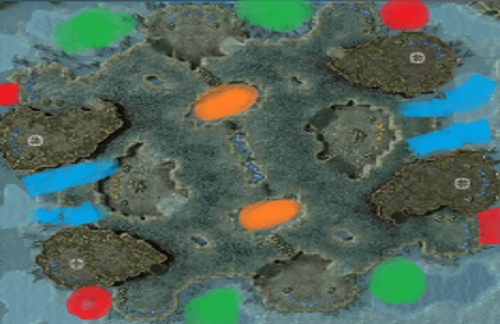
\includegraphics[width=.9\linewidth]{media/mapgeo.png}
    \captionof{figure}{Example of StarCraft map showing the geography}
\end{center}

\subsection{Clustering Map Data}

We will first determine the win/loss for each race’s matchups and try to find which general race benefits on 3 different sized maps. We will separate the maps into 3 main size categories: Small, medium, and large. By seeing which race benefits on each sized map we will be able to then go into more specific clustering and classifications to see what strategies implemented on those maps allow those races to have that win advantage.

\subsection{Small Maps}

Small maps typically imply that each player has to play at a pace much quicker than they would have to on a medium or large map. Expanding outside the initial base as soon as possible is key to avoid getting out-macroed, we will want to keep track of the number of bases each player has at every stage of the game. It is our prediction that rush strategies such as a "Zerg Rush" will be very common, and match length time will be significantly less than it would on a larger map scale.

\begin{center}
    \captionsetup{type=figure}
    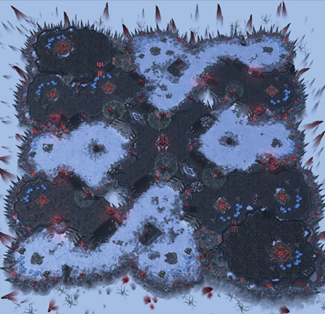
\includegraphics[width=.9\linewidth]{media/smallmap.png}
    \captionof{figure}{Example of small map}
\end{center} 

\subsection{Medium Maps}

Medium maps allow for a more balanced gameplay approach for each opponent, in theory this map size should represent a balanced win/loss rate per race and an abundance of different strategies and building decisions. It is our prediction that this will reveal our median match length time and provide no significant benefit to one race over another.

\begin{center}
    \captionsetup{type=figure}
    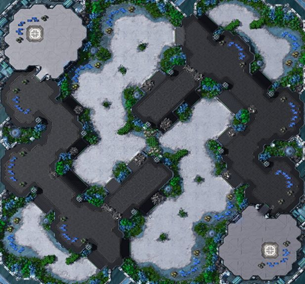
\includegraphics[width=.9\linewidth]{media/mediumMap.png}
    \captionof{figure}{Example of medium map}
\end{center}

\subsection{Large Maps}

Large maps are where strategies involving strong "macro-builds" will see the most in gameplay. Since the distance and expansion sites are large, this allows players to build up a strong economy. However, what is pivotal in these times of match ups is the success of pressuring or countering pressure, we predict that the match length should have an extreme variable of either mostly short- or long-lasting match times. 

\begin{center}
    \captionsetup{type=figure}
    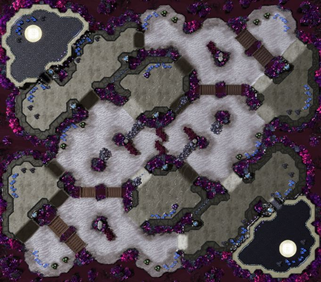
\includegraphics[width=.9\linewidth]{media/LargeMap.png}
    \captionof{figure}{Example of large map}
\end{center}

\subsection{Map Classification}

The data set we are using for the project is a selection of pro games over the course of 2018-2020. In pro games it is usual for the tournaments to have a set pool of maps that are played on for each given stage of the tournament usually around 8-10 maps and furthermore it is common for the overall pool to be shared across tournaments as certain maps provide a more balanced experience for 1v1 gameplay and the best experience to the players. Due to the shared map pool the total map pool when the replays were compiled at 30 maps.

\begin{center}
    \captionsetup{type=figure}
    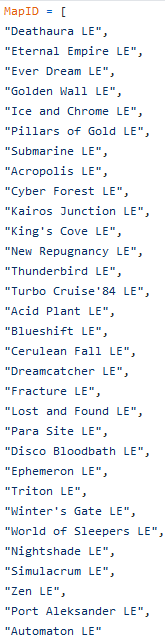
\includegraphics[width=.9\linewidth]{media/MapList.png}
    \captionof{figure}{Map List}
\end{center}

These maps are compiled into an array that stores each of the maps, then using the map information available from the map info which has been compiled by liquipedia it is possible to get the width and height of each of the maps in a number form of pixels. Ex.) DeathAura LE = 144 x 140. Pixels do not entirely give the full picture of map size but due to the maps having a low amount of extractable data from Blizzard this is what we found to be the most reasonable method of assigning a map size. Given the width and height, finding the area of the map and assigning that to a MapSize array was the next step and then appending the two maps together to make an array that mapped the ID of the map to the size. After assigning the maps there is a small algorithm to group each of the maps into evenly sized groups which essentially self classifies based off of relative map size where each map should be assigned.

\begin{center}
    \captionsetup{type=figure}
    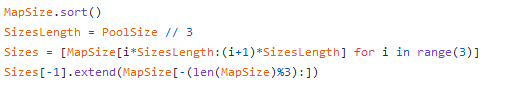
\includegraphics[width=.9\linewidth]{media/MapSorter.png}
    \captionof{figure}{Map Sorter}
\end{center}

Using this assignment algorithm it is possible to add to our data CSV the map area and a relatively small medium or large classification to be used later for win prediction. The role that map classification will ultimately play in the win prediction is for initial prediction using the ability to see a map size could be useful in helping shape which race should have the highest initial win percentage given any matchup.

\section{Micro \& Macro}
\subsection{Macro}

This section will focus on the macro Meta for StarCraft 2 and how macro effects the game of StarCraft 2. Macro is used commonly as a word for talking about large-scale effects or overall effects, StarCraft 2 is no different in this. In StarCraft 2 macro is often referred to as the overall state of the game and defining whether a player’s macro is good or not generally will refer to their overall control over the state of the game. It is important to define what goes into the overall state of a game to put a positive or negative value to it.

\subsubsection{Economy}

The core of StarCraft 2’s macro is balanced upon the economy system of the game, a system which at first appears to be simple. There are two primary resources of the game which are used for all macro decisions of the game, these are minerals and gas. Although it appears simple due to the lower number of currency options the macro complexity becomes rapidly complex when you discuss the varying ways to spend and acquire resources. The easiest way to explain the macro game would be to discuss the main ways to spend minerals and gas, these can easily be classified as Military, Technology, and Economy. Within Economy we have primarily ways of making more minerals or gas, this is new bases, workers, and gas collectors, all of these methods will boost the income in one way or another of the player meaning you have more to spend on Military, Technology, and Economy. Military is straightforward this is anything related to the defense or offense of the player with it primarily being buildings to build attack units and the units themselves which also cost resources to build.

Finally is Technology this is the hardest to classify as it is differing across the various races and strategies and can change rapidly across games but generally technology refers to upgrades you can invest in that will make units or buildings more powerful for the rest of the game. With these three the gameplay of StarCraft 2 forms a pseudo system of checks and balances with each way of spending being effective to counter one another. In this way if a player is to invest too much in their economy they may be able to gather a large amount of resources very quickly but that means they are generally going to have a weaker military meaning they could be susceptible to attacks from a player who spent more offensively. A player who spent heavily on military may have failed to spend enough on technology meaning they may have more units but their units might be significantly weaker than someone with a smaller but more refined army.

Finally spending all money on technology upgrades will lead to more powerful buildings and units but the units and buildings are still needed to make use of those which raises the need for an economy and due to the nature of spending heavily on technology it can lead to getting heavily outpaced economically and falling behind as the game progresses. Due to each major way of spending being tied together it is crucial that a good balance is found for the strategy the player is currently pursuing and that the player can analyze what the opponent is doing and react accordingly. These core fundamentals can be used to map out different analytics that can be used for tracking winning strategies. For each of these major categories comparing the statistics to the time and the other player’s stats can help reveal how the macro of a game plays out.

Some interesting data points that can be analyzed for the military would be, area of the map revealed, first unit production time, units per minute, resources spent on military, and finally supply. Supply is a 3rd pseudo resource that is gained by building a certain type of building/unit and allows for more units to be built up to a cap of 200 supply, the reason why this would be one of the best winning statistics to analyze is that supply is not a one to one ratio with units. Any unit in the game can be worth between one and eight supplies with more powerful or effective units generally being worth higher amounts of supply, because of this it is often viewed as the main statistic that correlates to army strength rather than units built. This becomes exceedingly important once a deeper look at the different races happens as different races tend to build extremely varying unit counts but may have similar army supply.

\begin{center}
    \captionsetup{type=figure}
    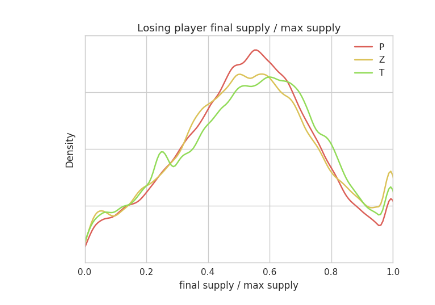
\includegraphics[width=.9\linewidth]{media/SupplyGraph.png}
    \captionof{figure}{Supply of losing player Source: “STARDATA: A StarCraft AI Research Dataset”}
\end{center}

When discussing the economy of the game the most important winning statistics to look at are the rates of acquisition of varying resources per minute. When looking at this statistic the race that the player is playing is also a key detail as some resources are more valuable for some races, for example zerg is generally considered a gas heavy race and thus will prioritize it for their mid to late game units whereas terran often will more heavily prioritize minerals. The other important economics-based stats to look at would be base improvement, this can be separated into two different parts buildings and workers. Workers are what is used to gather resources in StarCraft 2 it is important to note they can attack and be used to explore but generally the more workers produced the higher economical value a player will have. The other category will be the buildings that are gas producing buildings which are hard to quantify and number of bases owned, for each base a player is able to have a mineral field and two gas nodes. The number of bases expanded to is generally related to the map and the race but understanding the effects of base expansions can be an interesting note on winning strategies.

\begin{center}
    \captionsetup{type=figure}
    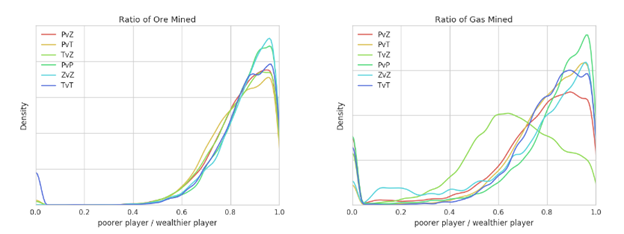
\includegraphics[width=.9\linewidth]{media/ratiogasoremined.png}
    \captionof{figure}{Ratio of Minerals and Gas Mined per matchup source: “STARDATA: A StarCraft AI Research Dataset”}
\end{center}

For Research it is exceedingly difficult to classify numerically how each upgrade has an influence versus another player as each race has their own research options of which they are varied and unique to certain strategies. Because of this it may be hard to use research timings to identify winning strategies, but it could be used to determine specific unit strategies and time these to winning strategies to determine their influence on the game.

\begin{center}
    \captionsetup{type=figure}
    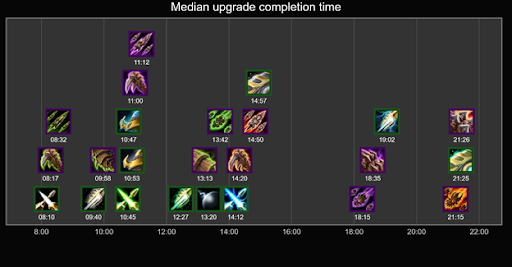
\includegraphics[width=.9\linewidth]{media/medianupgrades.png}
    \captionof{figure}{Median upgrade research time for zerg vs protoss matchups}
\end{center}

\subsection{Micro}

Micro in StarCraft 2 or micromanagement is generally referred to as the movements of units that can be used to reach victory.  Micro can be very complex within StarCraft 2 and the strategies involved will generally require large amounts of practice to master. Due to this level of mastery it may or may not be used within our winning strategy analysis, but it will still be outlined here. Most micro focuses around the control of military units specifically when trying to keep your units in an effective range where they can hit the enemies but can not be hit themselves or focusing the correct enemy.

The most commonly used statistic which could be used as a winning strategy would be to focus on the player’s APM. APM stands for Actions Per minute and refers to any movement selection or purchase a player makes. APM can be slightly misleading as spamming movements that are unimportant can lead to exceedingly high APMs, but unless it is being purposefully fooled by a player it will generally be correlated to how much control over each unit and building a player has. APM can be seen as a correlation to rank in a lot of cases with some pro players being able to reach 200-400 APM which may be four to five times the average player.

\subsection{The Balance}

It is pivotal that a player can actually balance these two techniques since it’s nearly impossible for a player to give full attention to both at the same time. One crucial feature in determining if a player can successfully manage both is to see their actions per minute or APM. More actions per minute may not guarantee that a player is able to produce a better macro or micro however, it is important to also recognize how many of those actions are "dead actions" or actions that don’t actually accomplish anything.

Knowledge of when to sacrifice micro for macro is another key component to an experienced StarCraft player, typically if a player is able to massively out macro their opponent then they will have a significant benefit due to their army size and upgraded unit composition. However two players who have the same typical macro skill level, those matches will typically come down to micro combat and positioning.

\section{Literature Survey}

\begin{enumerate}\setlength\itemsep{-.1cm}
\item A Few Useful Things to Know about Machine Learning
\item Deep learning: Introduction to deep learning concepts
\item Handwritten Digit Recognition with a Back-Propagation Network
\item Sparse autoencoder: Andrew Ng’s lecture notes
\item Attention Is All You Need
\item STARDATA: A StarCraft AI Research Dataset
\item StarCraft II: A New Challenge for Reinforcement Learning
\item Early Prediction of a Game Outcome in StarCraft 2
\item Grandmaster level in StarCraft II using multi-agent reinforcement learning
\end{enumerate}

\subsection{STARDATA: A StarCraft AI Research Dataset}

Although we will no longer be using this dataset, we can gather some insight from it. This paper explores the STARDATA dataset for StarCraft I: Brood War. As explained in the paper, there is more data about the Protoss race and also the \textit{Fighting Spirit} map. The data is broken up like the following.

\begin{center}
    \begin{tabular}{cccccc}
        \hline PvZ & TvZ & PvT & TvT & PvP & ZvZ \\
        18016 & 14531 & 17385 & 2550 & 7015 & 6149 \\ \hline
    \end{tabular}
\end{center}

We can see that Protoss games are more popular than any other. Therefore this dataset is somewhat unbalanced, but it does make up for it by its quantity.

This paper provides some of examples of learning and control tasks that can be addressed. Meaning that we can use some of these for our realtime win prediction engine.

\msection{Strategy Classification}

Strategy classification involves prediction of build order and other metrics. Although this task seems simple enough, we soon come into a wall when we realize that we're only receiving part of the information in realtime (fog-of-war), so we must address this issue first.

\msection{Inverse Reinforcement Learning}

This is sometimes called apprenticeship learning. Its defined as "the process of learning a task when given an expert trace but no explicit reward function" (Abbeel and Ng 2004). We do have the reward function of just winning a match, the smaller rewards between the beginning of a match and winning are very abstract. So, we must first research (or learn) a reward function for these specific scenarios.

\msection{Imitation learning}

Basically what most people think of when machine learning comes into mind. We attempt to create a black box that takes in current game state and outputs the best possible action at the current game state. But the issue with this, just like in strategy classification, is that we are only receiving part of all the information available in the game (fog-of-war).

\msection{Forward modeling}

In forward modeling we attempt to predict the future. Meaning that given the current game state we attempt to predict what will happen next. This is very useful for our realtime win prediction engine, since it is what it will essentially be doing.

\msection{Partial information handling}

There are several different methods of handling partial information. Heuristically, professional StarCraft gamers are very efficient in handling partial observations. These methods include: simply sending out scouts to uncover the fog-of-war, create a specific model whose task is to derive more information from partial information, use algorithms like particle filters or Kalman filters to estimate enemy position.

\subsection{Early Prediction of a Game Outcome in StarCraft 2}

"Early Prediction of a Game Outcome in StarCraft 2" written by David Leblanc and Sushil Louis from the Department of Computer Science and Engineering from the University of Nevada Reno, explores ways to predict outcome of a StarCraft 2 game, focused mainly on early game outcome prediction.

Since the focus of this paper is match outcome prediction for StarCraft 2, for our project Goal\#4, we would implement a supervised machine learning classification algorithm that can predict the outcome of a StarCraft 2 match given the current game state. We believe that this publication can give us an idea of where we can start and what other people have already done regarding this subject.

The paper starts with an introduction to what StarCraft 2 is, and the reasoning and importance of early game outcome determination. According to the paper there are 2 main reasons why being able to predict the outcome of the match early on is beneficial. First, it can help game balance designers understand the flow of the game and the reasoning behind a match outcome, which can help the designers keep the game interesting and challenging for players. Second, this information can also help players improve their own gameplay by knowing exactly when and what influenced their match outcome.

This also ties back to some of the impacts we believe our project will have. We are hoping with our results, we are able to provide game designers and game balancers of Everglades important information, so they can continue creating a fun and challenging real-time strategy video game.
Continuing with the paper, they defined their goals and also mentioned some previous work that has been done on StarCraft related applications already. One of the approaches is using a Bayesian model to predict the opening strategy of a player. There has also been game outcome prediction related work in the area of professional sports based on genetic programming, neural networks, and time-series history with multi-layer perceptron learning.

The approaches noted above, are only a few of the many that was presented in the publication, and they are the ones that we believe are the most associated with our own project. Our Goal\#3, identifying how map differences affect the output of games with similar strategies, requires us to first be able to identify the strategies from the players. The strategy chosen by the player might also be one of the metrics that can be used to predict agent performance, and this goes back to our Goal\#2, propose new metrics to predict agent performance. Since, strategy prediction was previously worked on using a Bayesian Model, it is something that we can definitely do some research on to see if it can also be applied for our project. As with the professional sports outcome prediction, most of the approaches seem very complicated for our level of knowledge. But neural networks are classification algorithms that we can try to look into.

The paper continues with the dataset that they utilized for their research. The data was collected in the form of game replays, and they collected these replays from professional tournaments, which they believe leads to the data being less noisy and more optimized for prediction. They also mentioned about the 6 types of possible matchups, but they will be only focusing on Terran vs Terran. The replay files’ information was exported to a text file which formatted an event as follows:

\begin{itemize}[,]
    \setlength\itemsep{-.1cm}
    \item Frame: The timestamps associated with the event. It can be converted into seconds.
    \item Player: The name of the player performing the action.
    \item EventType: The type of event or action the player performed:
    \vspace*{-2mm}
    \begin{itemize}[,]
        \setlength\itemsep{0cm}
        \item Build Event: Player builds a structure.
        \item Train Event: Player trains a new unit.
        \item Research Event: Player researches an upgrade.
        \item Ability Event: Player uses an ability.
    \end{itemize}
    \item General Action: Contains all mouse-click, hot-key, control groups, camera movements and other events.
    \item EventDetails: The details associated with that type of action. Is currently ignored for most part (Leblanc and Louis 3).
\end{itemize}

The data gets parsed and the events get sorted by time in a table called BOT (Build Order Table). This table is mainly used to count the units, buildings, research progress, ability events and APM (Actions per Minute) at any given point of the match. They also split the APM measure into Micro and Macro. With Micro being the ability and mouse click events, while Macro being the building, training, and researching events. After the features has been extracted, it is represented in a vector of attributes, and each vector serves as a snapshot of the game at a given time for a player.

This information is helpful for us in the way that it helps us have an idea of how to categorize our data. From their replays they were able to identify 5 categories of crucial information. We would definitely need a Frame, to keep track of the time that certain events happen. The EventType is also split up very nicely and covers events that could have an effect on match outcome. Having all our features at a given time in a vector could be a way for us to see how the game is going at a certain time and help us predict match outcomes. Though, this research paper focused only on TvT matchups, for our project we would like to look at other possible matchups as well.

Returning to the paper, they showed the outcome of their research and gave a warning that the assumption of the outcome of the game is the outcome for all features extracted could be incorrect. But they went ahead to learn whether a snapshot is likely to be a win or a loss. To do this, they fed the system with snapshots that contain the features and their associated outcomes. Since, the result is win or lose, they are able to do this with classifiers. They used a WEKA toolkit to evaluate the prediction accuracy of multiple different systems and Gradient Boosted Trees for determining confidence measures. They also used 70\% of the features extracted for training and 30\% for testing. The result was an average prediction of over 50\% of the snapshots during the early game. The earliest where they were able to predict all of the snapshots was after the match had been played out, and a prediction accuracy of 100\% at the last 4.9\% of the match.
Seeing how for our project, we are also trying to predict match outcomes, we would probably use a classifier algorithm as well to predict match output.

 Before this publication, not all of us were familiar with the WEKA toolkit. Some quick research shows that WEKA is an abbreviation for Waikato Environment for Knowledge Analysis developed at the University of Waikato, New Zealand. In short, "Weka is tried and tested open source machine learning software that can be accessed through a graphical user interface, standard terminal applications, or a Java API. It is widely used for teaching, research, and industrial applications, contains a plethora of built-in tools for standard machine learning tasks, and additionally gives transparent access to well-known toolboxes such as scikit-learn, R, and Deeplearning4j" ("WEKA"). 

We planned on using scikit-learn to perform most of our data analysis, but this toolkit could be beneficial for us to learn how to use, since it appears to already have a lot of tools built in regarding machine learning and that could help us create the machine learning classification algorithm that we need for Goal\#4. They also used Gradient Boosted Trees, which is a machine learning technique for regression and classification problems. Considering how we are also dealing with regression and classification; we can look into Gradient Boosted Trees as one of the possible algorithms to apply to our dataset. They split their testing (70\%) and training (30\%) set, we are definitely going to split our data into a training and a testing set as well. Looking at their research results, it appears that it is indeed very difficult to be able to predict early game match outcomes. It is probably due to losing players making good late game decisions that turn the match around or winning players making mistakes during the later phases of the match. Especially, since the replays are collected from tournaments, it is hard to determine which player is winning since both players are professional and can make decisions that can drastically change the outcome of the game. For our machine learning classification algorithm, we need to be able to predict match outcomes at any state of the game, including early game. Noticing how they did not achieve as high accuracy as they would have liked, it makes us wonder what we can do to improve upon that to develop an algorithm that can predict match outcomes at any given time with higher accuracy.

The last part of the paper talks mostly about what can be worked on in the future for their project that can maximize classification accuracy and minimizing over-fitting. It is also mentioned that their replays extractions were lacking some information such as, units, lots and income.
Perhaps, if we are able to collect more information regarding the state of the game at a given time, we would be able to have a more comprehensive vector/snapshot that includes more variables that have an effect on match outcome. Such as, the amount of resources, vision, damage dealt etc. This paper focused mostly on TvT matchups, to be able to give more general answers to our research goals like "characteristics that determine win" and "metrics that predict agent’s performance", we should look at other matchups as well.

In conclusion, this publication was a good read since it gave us some ideas of how researchers have already approached a similar problem. We were introduced to the toolkit and algorithms that they used, how they categorized and extracted their data from replays, as well as the accuracy that we can expect to get using the information that they have used.

\subsection{Approximation Models of Combat in Starcraft 2}

The goal of this paper was for the researchers to be able to predict specifically the outcome of a singular battle based on the complex and diverse armies that exist within Starcraft 2. This although being only a single battle is an extremely complex task as each unit has separate range abilities and movement meaning battles can not as easily be predicted by number of units or by the overall supply of the army but rather would have to be predicted using all factors at play in any given situation. Additionally, this paper aims to be able to predict the surviving number of units from the winning army in a full fight.

With Starcraft 2 having an extremely complex set of systems in play that make the game open ended it has become the target and testing ground for a lot of AI research and work, this paper explains how AI is mostly focused on the brute force angle of macro where they overwhelm less experienced players. This method of brute force however falls off with more experienced players able to completely game the AI by using superior micro and timing. The paper explains how each of the prior attempts have been made to make more challenging AI some using AI that can cheat or make use of info unavailable and some that don’t cheat but use imagery to actively decide game state. This paper goes on to state though that with all this research there is a lack of research on prediction of engagements with very few attempts made even at battle simulations.

This paper relies on some base assumptions which simplify greatly the prediction of engagements these are as listed: two armies, armies begin just out of sight, close clumping of units but random, attack move to begin the battle, and no micro management. One of the main focuses they decide as a stretch goal is the ability to predict micro management but all of these could become potential problematic errors when discussing the findings of a singular battle.

They practiced 3 different models for approximation titled $A_PX1$, 2 and 3 with $A_PX1$ being simultaneous perfect focus fire on a unit before swapping. $A_PX2$ being the same but with range simulated in giving a much larger benefit to ranged units as they now get free encountered attacks and finally $A_PX3$ being the same as $A_PX2$ but with attributes being accounted for in the model such as light armor and unit traits. Pictured below is the $A_PX3$ algorithm.

This code shows that even the more complex algorithms used for prediction were simplistic with most of the battle prediction coming down to a numbers game most likely of damage per second vs health count being the two important factors.

These algorithms they tested with 12 different compositions with increasing complexities to find how their prediction models stacked up versus the actual matchups, there were solid improvements in their finding as they raised the complexity of the models and comparing each model it is clear that having more available data in StarCraft is crucial to accurate prediction. One interesting point to notice is their use of smart targeting lead to less accurate modeling than the random targeting that the earlier models had used.

This paper highlights some limitations through their use of the combat model that are important to notice when working on our own models. Primarily the use of assumptions, from reading this paper any time an assumption is used in an RTS game it becomes extremely inaccurate, for example in this paper by assuming that armies are clumped it completely invalidates any data using units that have the ability to use AOE (Area of Affect attacks) for which they simulated several of these units and this may have lead to many of the inaccuracies experienced. In the use of data for win prediction within our data sets an example of how this could lead us astray is the overlord unit for zerg, this unit does not attack and has no abilities of note to use for combat but provides army supply to the zerg player if it was to be assumed that this was the only use we could safely cut overlord count from the models in order to further simplify the model. This would be an incorrect assumption though as sometimes the overlord is used to bait attacks or scout for the player despite its lacking stats.

The next major takeaway for model building from this paper is more info in a model generally is more beneficial. In the case of the models this paper used they saw significant increases in almost every improvement they made to their models as seen in the figure below $A_PX1$ to $A_PX2$ and $A_PX3$ made vast improvements with very little extra data added.

With this its easy to see how although the model will become more computationally complex every input can lead to a massive improvement in accuracy for our projects modeling we plan to use a much larger set of information for modeling and remove the unneeded or unhelpful information as we deem it unhelpful to improve the model. As can be seen negative impacts can also be found from having more complexity if one is not careful with their analysis of the impacts. In the case of $A_PX4$ the idea was solid with priority targeting but the implementation has to be perfect when incorporating very complex mechanics into a simple model, for this implementation to have been successful it would have needed to be perfectly mapped a priority of units based on current state and that itself could be an entire analysis paper due to the complexity of a problem as there is no right or wrong answer due to the open ended nature of the game.

\subsection{Use of Machine Learning Techniques in Real-time Strategy Games}

The goal of this paper is as described to rather than focus on the excessive amount of research in the field of automated gameplay focus on the prediction and analysis of scenarios in an RTS game that are overlooked or unorthodox. To do this as with much research and like the Everglades Analysis project, the choice of game to do all tests and research on is StarCraft for this paper. RTS games are famously great practice for machine learning and AI practice and StarCraft and its sequel are the prime RTS games, so this is a logical decision that many come to when doing initial research into these fields.

Starcraft is famously a very complex game and therefore it has spawned a diverse field of strategies as this paper explains over 180+ variations. Starcraft is especially known for having strategies that some would call unorthodox that only appear once in a while but without proper knowledge of a counter can be effective these have even gotten their own title being known as "cheese strategies" this paper aims to be able to predict these strategies prior to them happening as they are typically ignored in the development of AI for the game.
        	
This paper was extremely thorough in their preparation of analysis making sure to fully analyze the environment that they were working with before beginning any planning for their models and analyzing the challenges that are posed. Many of these challenges are shared with the Everglades Analysis Project as such it is interesting to see the differing tactics, we used to counter each of these. The first is the Expert Knowledge of the Game, in the case of the paper these researchers decided to take on an expert consultant to teach them the ins and outs due to the complexity level of identifying strategies this is a smart choice, for our project it was mostly learning through trial and error as code was built for each system everyone in the group would research what each unit does with some of the group having an understanding from having played the game a small amount in the past.

The second Challenge was the lack of a dataset this problem was solved by this paper through their use of bot vs bot games to collect large amounts of games, this has the error of being predictable and the bots being unrealistic in their playstyle for the Everglades analysis project there were three pivots made first from BWAPI data in a large unmarked set to another large set of anonymous games from Blizzard and then finally to the final dataset a more refined set of tournament games played within the last two years by pro players. Due to pro  players spending thousands of hours playing the game and theory crafting the best possible strategies for every situation we felt this was the most realistic data set that could be used.

The third challenge is the selection of features to use for the modeling in this challenge the research paper continued to use the advice of their consultants. On our side we made use of the diverse research papers that have been published over the years to see what was most commonly used within StarCraft machine learning to make up our CSV columns for our data. Finally the last challenge this paper ran into was the need to find strategies that they would identify using ones commonly seen in pro this was not a challenge for our project however as the goal is different and there was only one primary target for us, the winner.

Early Prediction for strategies used pro replays along with several different algorithms and eventually were able to predict with high confidence the build orders along with strategies that players in those games were employing. The next step of learning was collection of data using bots vs a collection of different players to eventually learn scouting and the ability to determine strategies based off of that scouting which is one of the core fundamentals of StarCraft.

This paper provides a breakdown of the server setup they used for training and processing using python and BWAPI shown in the figure below:

% img

As Seen in this image the setup that was made using a server to process the raw data that was being pulled from StarCraft in real time and then feeding it through their machine learning algorithm to train it and then coming up with their final score of the prediction to the strategy at hand. Similarly the proposed setup we have will look somewhat similar with our data set and eventually live data being exported to our algorithms and giving a live prediction of the win rate based on that snapshot of the data set.

In this paper the researchers opted for a set of binary classification models due to them being more flexible when expanding the model and strategy for the future as well as having better performance as features are tuned in the future. Similarly, to us they used their dataset to establish a listing of attributes as well as their results. In this case they picked Random Forests Naïve Bayes and Gradient Boosting Tree which are all algorithms that we have considered in the past for the project and therefore they shared the implementation method of using sci-kit learn as the primary python library. The first step they took was to eliminate statistics that were not relevant to the training of the models they did this using the initial models and put in a graph below.

This is something that we should also look to implement within our CSV with the initial training of the models as some of the statistics picked may not be quite necessary for determining the winner of the match. Although this may prove some of the features are unneeded it should pan out very different as items such as race are unimportant to determining strategy since strategies are race unique a feature such as race is crucial in determining early win prediction along with map information.

Using the information they received from this training they were able to eliminate Naïve Bayes as it was significantly worse than the others and found that GBM performed well on almost every task especially as the amount of features increased. With the models of the

\subsection{A Few Useful Things to Know about Machine Learning}

Another helpful publication that we have read is "A Few Useful Things to Know about Machine Learning" written by Pedro Domingos from the Department of Computer Science and Engineering at the University of Washington. This article summarizes 12 important lessons that other researchers have learned regarding machine learning that is hard to find in traditional textbooks. It also focuses mainly on classification algorithms. 

Since the subject of machine learning is still new to most of us and we know that we are going to have to learn how to use machine learning algorithms in order to reach our goals, we believe this paper can give us some good tips and tricks in the area of classification and hopefully it can be useful in reducing the time needed for achieving ideal results in our analysis.

The paper starts off by explaining what a classifier is. "A classifier is a system that inputs a vector of discrete and/or continuous feature values and outputs a single discrete value, the class" (Domingos 1). It also talks about how there should be an input of training set samples with the corresponding output and a testing set to see whether the classifier is able to produce the correct output.

This gives us some idea of how we can approach our Goal\#4, implementation of a machine learning classification algorithm that can predict the outcome of a match. We can have our output (win or loss) be a discrete value, where  and , which is our class. We can input a vector of feature values such as unit count, resources count, APM (Action per Minute) etc. and hope that we can develop a machine learning algorithm that is capable of accurately predicting match outcomes. As for splitting the dataset, we would definitely do that so we can have a testing and a training set.

The first key lesson talks about the 3 important components that most machine learning algorithm is made up of, this includes:

\begin{itemize}[,]
    \setlength\itemsep{-.1cm}
    \item Representation: A classifier must be represented in some formal language that the computer can handle. Choosing a representation of a learner is tantamount to choosing the set of classifiers that it can possibly learn. This set is called the hypothesis space of the learner. If a classifier is not in the hypothesis space, it cannot be learned.
    \vspace*{-2mm}
    \item \begin{itemize}[,]
        \setlength\itemsep{0cm}
        \item Examples: K-nearest neighbor, Support vector machines, Naïve Bayes, Logistic Regression, Neural Networks, Bayesian Networks etc.
    \end{itemize}
    \item Evaluation: An evaluation function (also called objective function or scoring function) is needed to distinguish good classifiers from bad ones.
    \vspace*{-2mm}
    \begin{itemize}[,]
        \setlength\itemsep{0cm}
        \item Examples: Accuracy/Error rate, Likelihood, Posterior probability, Margin etc.
    \end{itemize}
    \item GOptimization: We need a method to search among the classifiers in the language for the highest-scoring one. The choice of optimization technique is key to the efficiency of the learner. It is common for new learners to start out using off-the-shelf optimizers, which are later replaced by custom-designed ones.
    \vspace*{-2mm}
    \item \begin{itemize}[,]
        \setlength\itemsep{0cm}
        \item Examples: Greedy Search, Gradient descent, Linear programming, Quadratic programming etc. (Domingos 1-2).
    \end{itemize}
\end{itemize}

It continues by pointing out how most textbooks overlook the Evaluation and Optimization components, which could be even more important than the choice of learner.
It indeed appears that the Evaluation and Optimization components do get overlooked very often, since we have a lot of research planned ahead but, most of them are focused on technologies that we can use for our project and the different types of Representation. Knowing that the other 2 components are equally, if not more important, it does make us aware that we should also be conducting as much research on evaluation functions and optimization of our classifier as well.
The second key lesson focuses on the importance of setting aside a testing data set. It also gives a solution to insufficient data, which makes it costly to set aside data for testing instead of using it for training. This is called cross-validation, "randomly dividing data into (say) ten subsets, holding out each one while training on the rest, testing each learned classifier on the examples it did not see, and averaging the results to see how well the particular parameter setting does" (Domingos 2). It also makes a point that the fundamental goal of machine learning is generalization.

Though we have already planned on having our data split into training and testing sets, and we are likely going to have a large amount of data, this is still useful information to know. Perhaps, when we are going to practice using the machine learning algorithms with a smaller dataset before our actual complete dataset, cross-validation could be a useful tool for making the most out of the dataset that we will have.

Continuing with the third key lesson, data alone is not enough. It talks about no matter how much data you have; it is still not enough. He also mentions the "no free lunch" theorems formalized by Wolpert. Wolpert’s theorem states that no learner can beat random guessing over all possible functions to be learned. Machine learning can often do very well with general assumptions like similar examples having similar classes. It also works by induction rather than deduction which requires less input knowledge to produce useful results. One of the key criteria for choosing a Representation is what kind of knowledge is easily expressed in it.

This reminds us that even though we believe we are going to be able to collect a large amount of data, it is still not going to guarantee us a high accuracy classifier. What we need to focus on is choosing the right Representation based on the data that we are going to train and test. We planned on going over some of the most common machine learning algorithms such as Logistic Regression, K-nearest Neighbor, Naïve Bayes, Mean-Shift etc. in an attempt to understand them better so we know exactly which Representation will work best with the dataset that we will have.

Key lesson number four goes over the issue of overfitting. A big problem of machine learning is overfitting, that is when we do not have enough knowledge to be able to correctly determine the class, we can run the risk of making up a classifier that is not real and is just encoding random traits in the data. We know that we have a problem with overfitting, if the classifier does very well on the training set but poorly on the testing set. It mentions how we can use bias and variance to understand overfitting. "Bias is a learner’s tendency to consistently learn the same wrong thing. Variance is the tendency to learn random things irrespective of the real signal" (Domingos 3). The paper gives some methods to overcome the problem of overfitting. Such as, cross-validation, regularization term, and chi-square test. It also warns us that overfitting is not always caused by noise in the data, it can occur even in the absence of noise.

Learning that overfitting is such a large issue for machine learning, we will keep an eye to make sure that our classifier is not only doing well in the training set but, most importantly, it can accurately predict the correct class even with data that it has not seen beforehand. In the unfortunate situation that we encounter the overfitting problem, we now have some idea of how to combat this issue.

Fifth key lesson is about the next biggest problem in machine learning, dimensionality. Being able to generalize correctly becomes a lot harder as the number of features grows. It cautions us to be mindful of how many features we are gathering, because having more does not equal a better classifier, it could instead be outweighed by the problem of dimensionality. To combat this problem, we can use algorithms that are explicitly for reducing dimensionality.

Understanding that more features does not mean a better classifier is an important reminder. It might be a good idea if our classifier does not predict with our desired accuracy, to instead add one feature at a time and make sure that the feature to be added is statistically significant in predicting game outcome. This way, we could possibly avoid the problem of both dimensionality and overfitting. The paper did not mention what the dimensionality reducing algorithms are, but a quick search shows us that there are plentiful out there. For example, classical scaling, isomap, local linear embedding etc. which all seems very complicated and intimidating. Nevertheless, if we do come across a dimensionality problem during our data analysis, we would surely explore these algorithms further.
Moving on to the sixth key lesson, it is about theoretical guarantees. According to the paper, the main role of theoretical guarantees in machine learning should be a source of understanding and driving force for algorithm design, not as a criterion for practical decisions.

Probably the point of the seventh lesson for us, is to take guarantees with a grain of salt. The numbers can look good on paper but not be practical, or vice versa, the numbers can look less than ideal but it does not mean there are no practical uses for it.

The seventh lesson covers why some machine learning projects succeed and some fail. The difference between those two is mostly due to the features used. Most of the effort in machine learning projects goes to constructing features from raw datasets that are ready for learning. The publication makes it clear that a lot of time will be spent on gathering, integrating, cleaning, and preprocessing the data as well, and less time than people usually think on actually doing machine learning stuff.

This might have come as a surprise to some of us who have not had much experience with machine learning. With this knowledge, we might have to allocate more time and start earlier for the data collection and preparation process since it is apparently one of the most time-consuming part of a machine learning project.

Carrying on with the eighth key lesson, it talks about how more data can lead to a better classifier than more sophisticated algorithms. It points out that using a cleverer algorithm might not lead to the results we believe it will. Because in the end, they all do the same thing. All Representations basically tries to group nearby examples into the same class, the only difference between the algorithms is what is meant by "nearby". The author recommends us to start by using the simplest algorithms such as Naïve Bayes and K-nearest Neighbor. This is due to cleverer learners are harder to use and harder to get good results. There are also algorithms that have a fixed size, meaning they can only take advantage of so much data. Variable-size learners does not have that limit and can learn any function if given enough data. But then we are presented with the problem of algorithm limitations, computational cost, and dimensionality.

Taking the advice from this paper’s author, we are certainly going to start off our machine learning classification algorithm with the simplest Representations available and build up from there. Since, we were also introduced to fixed-size and variable-size learners, we should keep that in mind when we are using the different algorithms and understanding their limitations.

The ninth key lesson is about learning many models. Researchers noticed instead of choosing the best variation we can just combine many different variations, and that can actually lead to a much better result. This is called model ensembles and is what most researchers are doing nowadays. It mentioned some of the most simple and common techniques used:

\begin{itemize}[,]
    \setlength\itemsep{-.1cm}
    \item Bagging: We simply generate random variations of the training set by resampling, learn a classifier on each, and combine the results by voting.
    \item Boosting: Training examples have weights, and these are varied so that each new classifier focuses on the examples the previous ones tended to get wrong.
    \item Stacking: Outputs of the individual classifiers become the inputs of a higher-level learner that figures out how to best combine them (Domingos 7).
\end{itemize}

Since it appears that model ensembles are a standard for machine learning, we would probably have to learn more about these techniques mentioned above so we can see if this is a possible application to our dataset. Bagging does appear to be simple and doable and could be used for our project in hopes of having a classification algorithm that can predict match outcomes at a higher accuracy.

Proceeding with the next key lesson, simplicity does not imply accuracy. If we have two classifiers who have the same training error, it is believed that the simpler of the two will have a lower test error, but that is not always true. Complications can arise due to few learners searching their hypothesis space thoroughly. The size of the hypothesis space is a rough guide to the procedure by which a hypothesis is chosen.

The term hypothesis space has been used several times throughout this publication without a clear explanation. Just to be sure, "The hypothesis space used by a machine learning system is the set of all hypotheses that might possibly be returned by it" (Blockeel). We understand that choosing the simplest models might not give us the highest accuracy. We would be careful not to choose our model only based on simplicity.

The eleventh key lesson is another warning about implication, more specifically representable does not imply learnable. The author brought up the issue that simply because a function can be represented does not mean it can be learned as well. Given that we have a finite amount of data, time and memory, the algorithms will always only be able to learn from a small subset of all the possible functions that exist. Furthermore, since variable-size learners do not have a limit and can technically learn any function if you provide it enough data, answering the question that it can be represented. But the bigger problem is, is it learnable? Finding the solution to this problem is currently one of the major researches being done on machine learning.

Even though we will have a lot of data, it is still not going to be enough. StarCraft is such a complex game that it is not possible to teach our classification algorithm all the possible functions that can exist. We understand it is learning from only a subset of all possible functions and therefore we would never be able to achieve a 10\% accuracy. But we are hoping with enough research, trial, and error, we are able to implement a machine learning classification algorithm that can predict match outcome with a 7\% accuracy or higher.

The last lesson points out that correlation does not imply causation. It reminds us that correlation is a sign of a potential causal connection that requires further investigation and should not be treated as representing causal relations.

This last lesson is perhaps one of the most common sayings in data analysis. But it is still a good reminder that just because an independent variable that we found might be correlated to the dependent variable, it still does not necessarily mean one causes the other. This is something we need to keep in mind, as we are finding our characteristics and metrics for our analysis goals.

All in all, this publication shed light to a few new pieces of information. As well as reminders of information that we already knew. It appears that machine learning is a complicated process and there are many things we need to be wary of such as overfitting and the problem with dimensionality. New representations and techniques were provided, which we can further explore. Solutions were also given to some of the more common machine learning problems, giving us an idea where to start if we do encounter them.

\subsection{Predicting the Winner in 1v1s}

The goal of this paper is very closely aligned to the goal of the Everglades Analytics Project’s overall goals. The primary goal being to use statistics to determine winning strategies in RTS games and be able to predict a winner with a high rate of accuracy even from early into a match. Additionally, with this project  they have chosen the same RTS game as a base for their studies in StarCraft.

This paper decided to use StarCraft Broodwar as at the time that was the most relevant RTS to their studies rather than the StarCraft 2 the current project has pivoted to. This does not make a huge amount of difference when analyzing their paper in regards to finding meaningful research but does put a mark that anything they found must be translated to a more likely complex version for using StarCraft 2.

The Primary Study performed here is the setup of two AI that were both playing terran in order to have them play an even matchup against one another, to keep the matches even more even if the games were played on a single symmetrical map. The data from these AI matches were collected until the researchers had a perfect set of 100 games with each AI having exactly a 50\% win rate for a symmetrical dataset. This specific research went wide with their definition of important winning statistics using traces of different parts of the game they organized into a vector of 28 length in order to capture each unit building and resource type present for each player. 

The next part of the paper focused on their analysis using machine learning algorithms specifically Classification algorithms. Again being a smaller simple sample set the idea was to test on a small sample set a number of different classification models so as to locate the most efficient one. The algorithms chosen were LDA, QDA, SVM, KNN, and KKNN. Running each algorithm and analyzing the results led their research to find QDA as being the highest base accuracy of all of these, but go on to explain how the base accuracy is unimportant in a situation with a very even matchup and low variance is a crucial stat. Analyzing Variance allows them to see how with low amounts of games the "lazier" algorithms such as KNN and KKNN are strong but in larger sets greater than thirty nothing comes close to the accuracy provided with LDA.

This work is highly applicable to our project despite differences in data collection and depth of complexity. Most importantly this was a great kickstart to the process of identifying our models once we started to break down our preliminary data sets. Even having an analysis like this to serve as a basis despite differences allows to see some results that would surely be similar in the use of some of the classification models. This project helped realize how it is important to analyze win prediction on a matchup vs matchup basis versus an overall look as the Everglades project will not only focus on the Terran vs Terran matchup but rather all 6 possible matchup combos that can occur in the game. This also put the possibility of working with LDA and QDA into the forefront as there was no prior experience in the team with these. 

\subsection{Identifying Players and Predicting Actions}

This paper focuses less on winning strategies within RTS games but more on prediction of singular actions that a player has made. Although our project focuses primarily on the full win prediction an analysis of predicting any movement in an RTS game could be a sub part of the overall prediction of a game. 

This paper opens with a similar prompt to that of the project in that any advancement in AI and learning from an RTS game is highly applicable to uses in other RTS games and efficiency of other applications that can make use of strategy. RTS AI can be highly complex as explained and the complex nature of these games completely ruins the possibility of simplistic learning algorithms being usable for prediction. This paper specifically uses WEKA toolkit to apply machine learning algorithms to StarCraft 2 and manages to nail a fairly high action prediction rate given the wide variety of actions that can be performed. Due to this being an older paper StarCraft 2 was at the time of writing a rather new game having been used not very often in research and lacking in tools for replay extraction this forced the authors to have to be very resourceful with differing tools to clean their dataset and assemble a dataset of 2110 games, some of the same places they managed to acquire replays from were useful for us in the search for our DataSet as we transitioned off of Blizzard’s anonymous dataset to a set that worked with SC2Reader of pro games. 

This paper primarily focused on the use of ANNs or Artificial Neural Network, Random Forest, Adaptive Boosting, and C4.5 Decision Trees in order to apply machine learning. Using each of these methods on a number of features and characteristics that they extracted specifically related to the build order of units in these matches. One cool finding they found using pro game data is that using data they were very easily able to use the different playstyles that pros used and that further using that and APM it became possible to specifically target and identify pro players by name from the data set even going as far as always being able to narrow down the player to 2 or 3 when talking about similar players. When discussing their action prediction the paper explains that their initial action prediction was quite low but increases as the game progresses, this is due to a decrease in the amount of actions that are required later on.

This paper is a good look into Neural Networks and J48-C4.5 Decision trees as those had been not yet considered for our project. Looking specifically it is interesting to see how robust J48 was at being able to predict not only actions but also specific players. This paper is extremely applicable to the Everglades Analytics project as it uses StarCraft 2 and pro data in a similar way. It could be a good consideration for win prediction to first analyze action prediction to optimize.

\section{Machine Learning}
\subsection{Supervised Learning}

Supervised learning is one of the most popular algorithms that is used in machine learning. You have input variables and an output variable  which you want to be able to predict using the input variables. The goal of this is to generate a function that can map the inputs to output so well, that when we give it new data, it is able to predict the output variable. Supervised learning can be categorized into two types of problems. A classification problem or a regression problem. We will dive deeper into what are classification and regression problems, as well as demonstrate and explain some of the most common algorithms used to solve these types of problems. Supervised learning is going to be important for us since we are trying to create an algorithm that can predict match outcome using a set of input variables that we found statistically significant.

\subsection{Unsupervised Learning}

Unsupervised learning also has input variables  but they do not have an output variable . The goal of this is to model the underlying structure or distribution in the data in order to learn more about our data. Or in other words, we use unsupervised learning when we want to explore our data and find hidden patterns without having labeled responses. This is usually used to solve clustering problems, which we will also further explore and demonstrate some of the most common algorithms under clustering. We believe that we will be using some of the clustering algorithms mainly for discovering map differences. Which is important for our Goal\#3, identify how map differences affect the output of games with similar strategies.

\subsection{Reinforcement Learning}

Reinforcement learning is training an agent to make a sequence of decisions to achieve some goal that we have set. In order for the agent to make the correct decisions, it gets rewarded or penalized based on the action it took. We do not program the agent to take these actions specifically but, instead we allow it to learn what it should and should not do through trial and error. The agent usually starts with completely randomized actions and slowly it learns what actions give rewards and what actions give penalties.

Our project does not involve building an agent for our senior design project, we are simply trying to find characteristics and metrics that can determine win rate and player/agent behavior. As well as, understanding how map behaviors affect game outputs with similar strategies and implement machine learning classification algorithm that can predict match outcomes. Even for our stretch goal, which is to develop a real time analytics engine, it still does not appear to us that we need to build an agent that can make decisions in order to achieve our goals. Hence, for now we do not have any plans to further investigate reinforcement learning or creating an AI/agent, but if we discover that it is necessary or that it could be beneficial for our project in the future, we will delve deeper into reinforcement learning. For now, we are going to be focusing on Supervised and Unsupervised Learning.

% \section{Model Methodologies}
% \section{Real-world Applications}

\chapter{Design}
\section{Model Selection}
\subsection{Scikit-learn}

Scikit-learn is a Python machine learning tool for predictive data analysis. As part of our goals, we will use scikit-learn for classification, regression, model selection, and clustering algorithms to better gather our data to predict winning behaviors. Fortunately, the learning tool is built upon other mathematical libraries which play a part in discovering the information we need. Those libraries are NumPy, SciPy,Matplotlib, and Pandas.

\begin{itemize}[,]
    \setlength\itemsep{-.1cm}
    \item NumPy \\
    One of the most important and well-known packages to help support numerical computation allowing the use of matrices and arrays to help supplement any mathematical operation done on them.
    \item SciPy \\
    This package is dedicated to help with scientific computing, being built on top of NumPy this allows such features as linear algebra, optimization, image processing, and more.
    \item Matplotlib \\
    Is the library used in order to show the graphic and visualization side of the data that will be analyzed.
    \item Pandas \\
    This library allows the easy optimization of loading a dataset to use for the data analysis.
\end{itemize}

\subsection{Classification}

The main objective is to identify which class/category an object belongs to. In StarCraft this can be useful in the classification of strategies, based on unit and building orders we should be able to classify first if there is a theme of building defensively, overtly aggressive, or something balanced. Classification can be approached with these models: logistic regression, support vector classification (SVC), k-nearest neighbors, decision trees, and neural networks.

\subsection{Logistic Regression}

Logistic regression is one of the most common algorithms used for binary classification problems. Similar to linear regression, logistic regression tries to find an equation that can be used to predict the outcome, but the outcome is for a binary variable instead of a continuous one. It can also be used to describe data and to explain relationships between variables. Since the dependent variable in a logistic regression  has to be dichotomous, it can prove to be useful for predicting a StarCraft II match outcome, since the outcome can be a Win or a Loss. Logistic regression uses the logistic function, also known as the sigmoid function:
$$\text{sigmoid}(x) = \frac{1}{1+e^{-x}}$$
Therefore, to represent a model with multiple independent variables using a function we can have:
$$p = \frac{1}{1+e^{-(\beta_0+\sum\beta_iX_i)}}$$
Where $p$ is probability of the default class, $\beta_0$ is the constant/intercept, and $\beta_i$ is the coefficient for the $i$th independent variable. Even though logistic regression is mainly used for binary dependent variables, it is actually possible to use logistic regression to predict for multi-class dependent variables. In the case that there are more than two possible outcomes, a one-vs-rest (OvR) or one-vs-all (OvA) method can be used. This process splits the multi-class data set into several binary classification problems, which is then trained on each individual problem and the model that is the best performing will make the predictions. To demonstrate that this can be done using Scikit-learn, we will be using the famous iris data set.

The Iris dataset is available at the \link{https://archive.ics.uci.edu/ml/datasets/iris}{UCI Machine Learning Repository}, and it is also easily importable via Sciki-learn’s datasets. This data set has 150 observations, 3 classes: Iris-setosa, Iris-versicolor, and Iris-virginica, and 4 independent variables: Sepal Length in cm, Sepal Width in cm, Petal Length in cm, and Petal Width in cm. The goal is to use Logistic Regression to predict which class an unknown iris belongs to when given a set of independent values. Since there are three possible iris classes, Scikit-learn will be performing the OvR method. This will split our multi-class classification problem into three binary classification problems:

\begin{itemize}[,]
    \setlength\itemsep{-.1cm}
    \item Problem 1: Iris-setosa vs [Iris-versicolor, Iris-virginica]
    \item Problem 2: Iris-versicolor vs [Iris-setosa, Iris-virginica]
    \item Problem 3: Iris-virginica vs [Iris-setosa, Iris-versicolor]
\end{itemize}
 
Since we are required to use three different models, it could be a very slow model if we have a large data set. In the case that there are only two possible outcomes, this would not be a problem. In Figure 31, we can see that by calling LogisticRegression from Scikit-learn, the Iris data can be fitted, and we get a mean accuracy of 95.5\% for this model. 

\subsection{Neural Networks}

Neural networks can be considered supervised and unsupervised depending on how the problem is set up. It is a supervised learning algorithm if we know what the outcome is and want to use a neural network to classify and learn the correlations between data and labels. It is an unsupervised learning algorithm if we do not have the answer for what the outcome is, meaning we do not have labels for our data. If we decide to use a neural network as an algorithm for our senior design project, it will probably be used for classification. Neural networks contain layers that work together to learn patterns in the data set. The simplest neural network is called a perceptron or a single layer neural network, which contains an Input Layer and an Output Layer. It takes data input and produces a single binary output. Usually after adding the first input layer we add a hidden layer. Each node in these layers multiplies the input value by some weight and normalizes the output with an activation function. In Figure 32, we can see a basic input, output, and hidden layer neural network. 

The entire neural network process is long and complicated but luckily, Python has several libraries for neural networks that we can use. One example is the Keras API. After randomly generating some data we can import the necessary classes from Keras. Figure 33 shows that by using Keras we can create a simple input and output layer sequential neural network with the Sigmoid function as the activation function, the binary cross entropy loss function as the loss function, and Adam as the optimizer. Using Keras, we have control of how many layers we want to add to our neural network, as well as how many nodes on each layer, which activation function and loss function we would like to use. We can select our preferred optimizer and fit the model according to the number of epochs and batch size we would like. 

\subsection{Regression}

Regression is used primarily in being able to predict the value of some specific attribute for the desired object. In StarCraft we can implement this to predict the economy and "macro-ing" aspects of the game to see if one player will have a significant economical advantage over the other. However, since this is a real time strategy game (RTS) the economic strength of one player’s army can flip in the course of a single battle. Regression can be approached with these models: support vector regression (SVR), k-nearest neighbor, and Lasso Regression.

Regression analysis is a modelling technique that is used to understand relationships between the dependent variable and the independent variable(s). The dependent variable has to be continuous and it is the variable that is being tested and measured, such as life expectancy. Independent variables are continuous or dichotomous variables that has an effect on the dependent variable, such as gender (dichotomous) or income (continuous). The main point of using regression analysis is finding a mathematical equation that can be used to predict a continuous dependent variable ( ) based on some number of continuous or dichotomous independent variables ( ). It is also extremely useful in answering questions such as:

\begin{itemize}[,]
    \setlength\itemsep{-.1cm}
    \item Which of the independent variables have an impact on the outcome?
    \item Which of the independent variables matters the most?
    \item Do those independent variables depend on each other?
\end{itemize}

Regression analysis might prove to be useful for our project since we are attempting to find at least 5 characteristics or independent variables that have an impact on winning a StarCraft II match. Additionally, for our second goal, we are trying to find 5 new metrics that can be used to predict agent performance. Using regression analysis, we will be able to determine which of these metrics and characteristics has an effect on match outcome and performance, and how they relate with each other.

\subsubsection{Linear Regression}

Linear regression is one of the most common and simple analysis approaches used for predicting outcome of a dependent variable. As its name states, this regression is linear because all the terms in the model are either a constant or a parameter multiplied by some independent variable.
 
\msection{Simple Linear Regression}:

For a simple linear regression, meaning we only have one independent variable that has a linear relationship with our dependent variable, the least squares line equation is as follow:
$$y=\beta_0+\beta_1X$$
Where Yis the dependent variable, $\beta_0$ is the constant, $\beta_1$ is the regression coefficient for the independent variable $X$.
To find 0 we use the formula:
$$\beta_0=\bar{y}-\beta_1X$$
Where yis the mean y score and x is the mean x score. These can be calculated with the following equations:
$$\bar{y}=\frac{\sum_{i=1}^ny}{n}\qquad\bar{x}=\frac{\sum_{i=1}nx}{n}$$
Where n is the total number of observations. We also need to find 1 in order to find the least squares regression line for our simple linear regression. $\beta_1$ can be calculated with the formula:
$$\beta_1=\frac{SS_{xy}}{SS_{xx}}=\frac{\sum_{i=1}^n(x_i-\bar{x})(y_i-\bar{y})}{\sum_{i=1}^n(x_i-\bar{x})^2}$$
This would be a very tedious task to do by hand if we have a lot of data points. But, using Scikit-learn’s already available function LinearRegression() we can quickly find our $\beta_0$ and $\beta_1$ for the simple linear regression line.

To demonstrate how linear regression works and how we can use functions readily available from Scikit-learn to achieve this, we will be looking at a dataset from \link{http://www.espn.com/college-football/rankings}{AP Top 25 2018} College football rankings for week 8. Simple linear regression only has one independent variable and one dependent variable. So, for this example, we have chosen our dependent variable $(y)$ to be Points Scored per Game, and our independent variable $(x)$ is Passing Yards per Game.

We can first plot the scatterplot, which is useful in detecting visual evidence of linear relationship between the two variables. If there does not appear to be any visual evidence of linear relationship, then linear regression is probably not the right approach for this dataset. Figure 10 shows the $x$ values and $y$ values stored in arrays. As well as using the scatter() function from matplotlib, we get a visual representation of our datapoints. The scatterplot does appear to show that there exist somewhat of a positive linear relationship between the dependent and independent variables. 

Next, we would like to use Scikit-learn’s LinearRegression() function to find our least square regression line.

By simply calling LinearRegression() as shown in Figure 11 and fitting it with our independent and dependent arrays, we can get the value for $\beta_0$ and $\beta_1$. Therefore, our least squares regression line for this simple linear regression problem is:

What this can tell us is that for every one-yard increase in Passing Yards per Game, we can expect the mean Points per Game to increase by 0.0599. Now, that we have our regression line, we can use it to predict Points per Game. In Figure 12, we can see the data points and the linear regression line plotted. The line does appear to somewhat fit the points on the scatterplot. 

If a college football team has 145.5 yards per game, we can use our regression line to predict how many Points per Game this team will have, 

% img

Comparing this predicted result with the actual result 29.3, we can see that our model is doing pretty well. But, in order to determine whether a linear regression model is actually good or bad at predicting the dependent variable, we would need to do more than just comparing one observation or visually hypothesizing. A very common way of checking whether a model is sufficient in predicting the dependent variable, is the coefficient of determination or the $R^2$. This can also easily be calculated using Scikit-learn. 

% img

Figure 11 shows the $R^2$ value of $0.291$ for our college football example. This can be interpreted as approximately 29.\% of the variability in the Points per Game can be explained by this linear model containing Passing Yards per Game. Since we have the $R^2$ value, we can calculate the Pearson’s Correlation Coefficient:

Thus, for our college football example, we have $r=\sqrt{0.291}=0.54$. This tells us that there is a moderately strong positive linear relationship between Passing Yards per Game and Points per Game. Perhaps the low value for coefficient of determination in our example is due to the inconsideration for the other existing independent variables that may have an impact on the dependent variable. 


\subsubsection{Multiple Linear Regression}
If there are two or more independent variables that have linear relationships with our dependent variable, then it is considered a Multiple Linear Regression, with the formula:
$$Y=\beta_0+\beta_1X_1+...+\beta_k\beta_k$$
Where $Y$ is the dependent variable, $\beta_0$ is the constant, $\beta_1$ is the regression coefficient for some independent variable $X_1$. Since, for multiple linear regression we have more than one independent variable, the $k$ in the equation stands for the number of independent variables.

Returning to the college football team example, we can attempt to add more independent variables with the goal of improving our linear model. Apart from using the independent variable Passing Yards per Game, we will be adding two additional independent variables, Total Yards and Rushing Yards per Game to predict for Points per Game. Utilizing the same LinearRegression() function available from Scikit-learn that was used for simple linear regression, we can use it to perform a multiple linear regression. Figure 14 shows a new data frame with $X_1$, $X_2$, $X_3$, and $y$. Where $X_1$ is Passing Yards per Game, $X_2$ is Total Yards, $X_3$ is Rushing Yards per Game, and $y$ is the dependent variable, Points per Game. By calling LinearRegression() on the independent variables and the dependent variable, we get the constant and coefficients for the multiple linear regression line.
$$Y=-15.4618+.0939X_1+.0027X_2+.0908X_3$$
What this equation means:
\vspace*{-.9cm}
\begin{itemize}[,]
    \setlength\itemsep{-.1cm}
    \item For every one-yard increase in passing yards per game, we expect the points per game to increase by 0.0939, holding the other two independent variables constant.
    \item For every one-yard increase in total yards, we expect the points per game to increase by 0.0027, holding the other two independent variables constant.
    \item For every one-yard increase in rushing yards per game, we expect the points per game to increase by 0.0908, holding the other two independent variables constant.
    \item The constant means that when a college football team has zero passing yards per game, zero total yards, and zero rushing yards per game, we would expect the number of points to be -15.4618, which has no practical interpretation. 
\end{itemize}

Now that we have a multiple linear regression model, checking its $R^2$ value using Scikit-learn, we get 0.7354, meaning approximately 73.5\% of the variability in Points per Game can be explained by this new model containing Passing Yards per Game, Total Yards, and Rushing Yards per Game. Which is a significant increase from our previous simple linear regression model that only contained one independent variable. 

\subsubsection{Interaction Models}
When we have a relationship between our dependent variable  and one independent variable $(x_1)$ that depends on the value of another independent variable $(x_2)$, an interaction model would be appropriate. We can represent this model including interaction between $x_1$ and $x_2$ in a formula such as:
$$Y=\beta_0+\beta_1X_1+\beta_2X_2+\beta_3X_1X_2$$
Where $Y$ is the dependent variable, $\beta_0$ is the constant, $\beta_1$ is the regression coefficient for some independent variable $X_1$, $\beta_2$ is the regression coefficient for some independent variable $X_2$, and $\beta_3$ is the regression coefficient for the interaction term between the independent variables $x_1$ and $x_2$.

Continuing with the college football team example that we have been working with, we can further attempt to improve our model by including an interaction term. Similar to the previous example, we have three independent variables. Passing Yards per Game $(x_1)$, Total Yards $(x_2)$, and Rushing Yards per Game $(x_3)$, which we used to predict Points per Game $(y)$. In order to identify which of these independent variables may have interaction effects, we will take two independent variables and make one of the independent variables a boolean series. Which means if the observed value is larger than the median for that independent variable, we will label it as 1, and if it is lower or equal to the median value, we will label it as 0.

Python has a built-in library for descriptive statistics called statistics, which we can use to easily get the median value for each independent variable, as shown in Figure 15. After the boolean series are created, we continue by creating a scatterplot, plotting one of the independent variables against our dependent variable, and setting the hue to be the boolean series of the other independent variable. Python also has a data visualization library called seaborn that allows us to create scatterplots with hue (grouping variables that will produce points with different colors). If there appears to be separation between the colors in the scatterplot, then that could be an indication of interaction between those two independent variables. 

Since we have 3 independent variables, the possible interaction terms are:
\begin{itemize}[,]
    \setlength\itemsep{-.1cm}
    \item $x_1$ and $x_2$, Passing Yards per Game and Total Yards
    \item $x_1$ and $x_3$, Passing Yards per Game and Rushing Yards per Game
    \item $x_2$ and $x_3$, Total Yards and Rushing Yards per Game
\end{itemize}

Figure 17 shows the scatterplots for each possible interaction term. None of them appears to have a really sharp separation between the orange and blue points. Figure 18 shows an example of how a scatter plot would look like if there are strong visual signs of interaction between two independent variables.

For the sake of demonstration, we will choose which interaction term to further explore based on which of the three scatterplots seem to have the most separation between orange and blue, which appears to be $x_1$ and $x_3$, Passing Yards per Game and Rushing Yards per Game. Using a Python module called statsmodels, we are able to find the coefficients for our interaction model. The table shown in Figure 19, provides us with the coefficients necessary to represent our model in a formula.

Hence, our model to predict for Points per Game by using Passing Yards per Game, Total Yards, Rushing Yards per Game, and the interaction term between Passing Yards per Game and Rushing Yards per Game can be represented as below:
$$Y=-21.9477+.1119X_1+.0032X_2+.1270X_3-.0001X_1X_3$$
It seems that the interaction term for our model has a rather small coefficient. Additionally, Figure 19 provides us with $P>|t|$, the p-value which equals to 0.648 for the interaction term between $x_1$ and $x_3$. If the p-value is larger than , that means there is insufficient evidence to indicate that the term is useful for prediction.  is the significance level, it is the probability of rejecting the null hypothesis when it is actually true. Most of the time, the  value is 0.05 (\%) or 0.1 (1\%). Since, our $p-value$ 0.648 is larger than 0.1, we can say that at 1\% significance level there is not enough evidence to indicate that the interaction term is useful in predicting Points per Game. Just as we have previously checked the $R^2$  value for each of our model, Figure 20 shows the $R^2$ value for our model with interaction terms.

It is clear that adding the interaction term did not really increase our $R^2$ value. For the multiple linear regression, where we only used the three independent variables, without interaction terms gave us a $R^2$ value of 0.7354. Considering the small number of differences in the $R^2$ value, the interaction term itself failing a hypothesis test, as well as adding complexity to our model, the interaction term will not be included in our future models.

\subsubsection{Polynomial Regression}
The previous regression models were all assumed to have a linear relationship between the dependent variable and the independent variable(s). When a model is not a straight line but has curvature, we can consider polynomial regression. Polynomial regression is a regression analysis where the relationship between the dependent variable and the independent variable(s) are modelled as nth degree polynomial in the independent variable(s).
 
\subsubsection{Quadratic Regression}
Quadratic regression is also known as a second-order model, as its name states, this model includes an $x_2$ term. If our data is plotted and there appears to be a U shape or an inverted U shape, this could indicate that quadratic regression is more appropriate than linear regression. The equation for a quadratic model with one independent variable is as follow:
$$Y=\beta_0-\beta_1X+\beta_2X^2$$
Where $\beta_0$ is the intercept or constant, $\beta1$ is the shift parameter, and $\beta2$ is the rate of curvature for some independent variable.

Since, plotting the independent variables against the dependent variable for the college football team example does not appear to have a UU shape, inverted U shape or much curvature at all, as seen in Figure 17 previously, it is likely not appropriate to use quadratic regression. Therefore, we will be using a new dataset, \link{https://online.stat.psu.edu/stat462/node/159/}{Yield dataset}. This Yield dataset contains measurement of yield from an experiment done at different temperatures. We have our dependent variable Yield $(y)$ and our independent variable Temperature $(x)$ in Fahrenheit. Figure 21 shows the dataset as well as the scatterplot. There appears to be some curvature in the scatterplot. So, we can continue attempting to run a quadratic regression analysis on this dataset.

To find the coefficients for our quadratic model, we can use the Python module statsmodels, similar to what was done for our interaction model example. 

Figure 22 gives us the coefficient for $\beta_0$, $\beta_1$, and $\beta_2$ and their p-values. Since the p-value of temperature squared is 0.001, which is smaller than 0.1, we can say that at 10\% significance level there is sufficient evidence to indicate that temperature is curvilinearly related to our dependent variable, Yield. So, for the Yield data set our quadratic model is:
$$Y=7.9605-.1537X+.0011X^2$$
Using Python’s maplotlib, we can plot our quadratic regression model line onto the scatterplot and visualize how our line looks, as shown in Figure 23. 

As always, checking the $R^2$ value for our current model, we get a value of 0.6732. Meaning approximately 67.3\% of the variability in Yield can be explained by our current quadratic model. 

\subsubsection{Higher Order Regression}
Higher order regression usually refers to when the relationship between the dependent variable and the independent variable(s) are modelled as third-degree polynomial or higher in the independent variable(s). A third order model is also known as a cubic regression model. The function for a cubic regression model is:
$$Y=\beta_0+\beta_1X+\beta_2X^2+\beta_3X^3$$
We may technically also be able to have $n - 1$ order regression model, where n is the number of data points. But most of the time it is better to keep the order/degree of the regression model as low as possible, such as a first-degree polynomial, also known as linear. If necessary, a second-order polynomial can be tried, also known as quadratic. If a lower order of polynomial is not satisfactory, we may try higher order for the model function. Using higher order regression requires more factors, which not only makes the function more complicated, but it can also lead to overfitting.

Meaning, the model learns too many details and noise from the training data to the point that it loses the ability to generalize. This causes it to appear as if the model is doing good on the training set but, when tested on the testing data set, the performance will be poor. Practically, models higher than a third-degree polynomial are not often used. Below is a table that displays the number of variables needed for different orders of regression, with  being the number of independent variables $(x)$.

Since the first step of fitting a regression model to a dataset is plotting a scatter plot to see the shape of the data. In Figure 25, we can see an overview of how the graph of different degrees of polynomial looks like, which we can then use to compare our data set’s scatter plot and see which one it seems to fit the best. 

\subsubsection{Lasso Regression}
Lasso Regression is also known as the Least Absolute Shrinkage and Selection Operator. It is a type of linear regression that focuses on shrinkage and can also be considered a simple technique used to reduce model complexity. Shrinkage means the data values are shrunk towards a central point, such as the mean. It also shrinks the less important features’s coefficients to zero, hence some variables can be removed, creating a simpler regression model. Lasso Regression is appropriate for models that have high levels of multicollinearity. 

Multicollinearity is when two or more independent variables are highly linearly related. It uses a technique called $L1$ regularization. Regularization is used to solve the problem of overfitting, which is a common problem when there is a large data set with a lot of features involved. $L1$ regularization adds a penalty that equals to the absolute value of the magnitude of the coefficients to the loss function. The Lasso Regression’s loss function is:
$$\sum_{i=1}^n\left(y_i-\sum_{j=1}^px_{ij}\beta_j\right)^2+\lambda\sum_{j=1}^p|\beta_j|$$
Where $n$ is the number of data points, $p$ is the number of independent variables, $x_{ij}$ is the value of the $j$th variable for the $i$th data point, $\beta_j$ is the coefficient for the $j$th variable, and $\lambda$ is the tuning parameter, it controls the strength of the $L1$ penalty, or it can also be known as the amount of shrinkage. If we set $\lambda$ to zero, parameters will not be eliminated, and it will basically be a regular linear regression. If we increase $\lambda$ the bias will increase and more coefficients will be set to zero, ultimately eliminating some parameters from the function. Scikit-learn has the option for Lasso under linear\_model, which can be used to fit a model for a data set using Lasso Regression. Returning back to the college football example as demonstrated in the linear regression section of this design document. As shown in Figure 26, if we set the or value to zero, we get a basic linear regression. The intercept, coefficients and $R^2$ values are all the same as a linear regression. 

If we increase $\lambda$ the value, some of the parameters might be shrunk to zero, which causes them to be eliminated from the function. Figure 27 shows the intercept, coefficients, and $R^2$ values for $\lambda=0.3$.

The independent variable $x_3$, Rushing Yards per Game has a coefficient of 0, which yields us the function:

Meaning the independent variable  can be removed from our function. This led to a lower $R^2$ value in this specific example. But when we have a data set with a lot more independent variables than just three, we might want to cut down the most irrelevant ones in order to keep our model simple and avoid overfitting, this is when Lasso Regression will really prove to be useful. 

\subsubsection{Ridge Regression}
Ridge Regression is also a type of linear regression that is similar to Lasso Regression. It uses a type of shrinkage estimator that is called the ridge estimator. This ridge estimator creates new estimators that are shrunk to be closer to the true population parameters. Similar to the Lasso Regression, the Ridge Regression is also appropriate for dataset that have a lot of multicollinearity. The main difference between those two are the penalty term in the loss function. Lasso Regression adds an absolute value of magnitude of coefficient as the penalty, meanwhile Ridge Regression adds a squared magnitude of the coefficients as the penalty term. This is called the $L2$ regularization, which gives us the Ridge Regression’s loss function:
$$\sum_{i=1}^n\left(y_i-\sum_{j=1}^px_{ij}\beta_j\right)^2+\lambda\sum_{j=1}^p\beta_j^2$$
Since for the Ridge Regression, the coefficients are all shrunk by the same factor, none of them will be eliminated, unlike the Lasso Regression that can reduce the model complexity by removing some variables. Here, when  equals zero, the Ridge regression is the same as least squares regression. If $\lambda$ is infinity, then the coefficients are shrunk to zero. Therefore, Ridge Regression is a better technique when the data has features that we know are relevant. Ridge Regression is also easily applicable by using the Ridge feature under Sciki-learn’s linear-model class. Figure 28 shows that when $\lambda=0$, Ridge Regression results in the exact same intercept, coefficients and $R^2$ value as linear regression would.

If we increase $\lambda$ to 0.3, as shown in Figure 29, we can see that the coefficients got shrunk towards zero but, none of them has been eliminated as with the Lasso Regression. 

If we increase $\lambda$ even more, for example to $\lambda=10$, we can see in Figure 30, that the coefficients got pushed towards zero even more, but none of them is actually zero. Meaning we are not able to eliminate any of the variables completely, but by being able to shrink the coefficients closer to zero, this will lead to a model that can perform better on unknown data sets. 

In general, the Ridge Regression and the Lasso Regression are both great techniques when dealing with data set that has a lot of features and/or multicollinearity, and we know that for our StarCraft II data set, we do indeed have a lot of features.

\subsection{Clustering}
Clustering is the grouping of objects into similar sets, this is a form of unsupervised learning and can give us a more general idea of insights and metrics that group and not so much predicting. One specific example of how this can be applied to our StarCraft analysis is classifying which race performs better on which specific map. Some algorithms correlated with classification is: k-means, mean-shift, and spectral clustering.

\subsubsection{Handwritten Digits Classification Example}

Included with the Scikit-learn library are multiple toy datasets intended on teaching users the basics to Machine Learning analysis with data that doesn’t need much preparation before being trained/tested.

One of these included datasets are a group of pixelated numbers that represent "handwritten digits" and by using SVC as an algorithm to classify the digits, we can train a model to predict what the numerical value of the handwritten digit is.

\msection{Loading the dataset}

Each of the data points represent an $8_x8$ image of a digit, using pandas we can see the shape of the data frame and the raw image data:
The image pixel color shade is what determines the integer value from 0-16. The range is white = 0 all the way to black = 16. Shades of gray fills in the gaps 1-15. These arrays makeup how the actual image would look in an integer form.	

This tells us that the shape of our dataframe is $(1797, 64)$, there are 1797 instance samples, and 64 attributes to each sample
The actual data attributes look like this:

% img

We see that since each instance has 64 attributes in the range 0-16, this makes up the general look of the number. Our target attribute will show the actual numerical value of the digit, which is used to train the model to predict the numerical value:

% img

This will output the corresponding numerical values of all 1797 samples: $[0, 1, 2, ..., 8, 9, 8]$. So the first digit is a 0, next is a 1, and so on all the way to the last digit being 8.

From here we will be using the SVC algorithm to train and eventually test that model using the last few samples. Typically we would use train test, split however in this example we will manually see how the prediction works by saving the last two images to check manually if the prediction is correct.

\begin{itemize}[,]
    \setlength\itemsep{-.1cm}
    \item We first create the actual SVC model with the basic inputs of $\gamma = .001$ and the regularization parameter = 100, we can edit the $C$ value based on data pool size.
    \item We then initialize our X variable attribute data set and y target data set, we want to use all of the samples, except the last two digits to test our model after fitting it.
    \item Calling the fit method, this creates the "learning" foundation of the model, this will hold all but the last two samples.
\end{itemize}

\msection{Scikit-Learn Predictor and Estimator Functionality}

We will now see if the prediction part of the model will be correct, Scikit-learn has a method called predict in the SVC object that takes the previously fitted graph and uses the new data to predict what the intended target value should be:

% img

We get the following output:

% img

We can look at our target data set to see if its correct, or we can print out the actual picture of the digit and see manually if the prediction was correct as below:

% img

By changing the value digit.images[-2] to digit.images[-1] and we get the two following pictures:

% img

Comparing those two images with our predicted output we can see that our model has successfully predicted the last two digits in the dataset. We also have the ability to make our own datasets if we really wanted to test the accuracy of this model.

\msection{Evaluation Functions}

Evaluation is how we can distinguish between a good and a bad model. It is how we can choose which model we prefer over the other models. It is also known as loss function, scoring function, utility function etc. This is important since we will be generating different models and we will need a way to decide which one is the best. Understanding what the options are for evaluating models and the pros and cons for each metric, we will be able to make the best decisions for our dataset. Some of the most common evaluation functions are:

\msection{Accuracy}

Accuracy or Classification Accuracy is the fraction of prediction that our model got correct.
$$\text{Accuracy}=\frac{\text{Number of correct predictions}}{\text{Total number of predictions}}$$
An accuracy close to 0 means our model performed very badly, and an accuracy close to 1 indicates that our model did a great job. But accuracy is not a good metric to assess our model’s performance if we have a dataset that is very imbalanced. For example, if we have a dataset that has 9\% of its sample from class A and only \% of the samples are from class B. Even if our model predicts every new data point as class A even when we have datapoints from class B, the accuracy will still remain high, giving us a false illusion that are model works. Accuracy is not difficult to calculate, scikit-learn has an accuracy function available, accuracy\_score.

% img

In Figure 1, we can see an array called y\_pred that has our predicted classes and y\_true is the true label for these samples, and by simply calling the accuracy\_score function we get an accuracy of 0.83, which is pretty good.

\msection{Mean Squared Error}

Mean Squared Error (MSE) is the sum over all the datapoints, of the square of the difference between the actual and predicted output divided by the number of datapoints.
$$MSE=\frac{1}{n}\sum_{i=1}^n(y_i-\hat{y}_i)^2$$
Where $n$ is the total number of datapoints, $y_i$ is the actual output $\hat{y}_i$ and  is the predicted output by the model. The $MSE$ is most commonly used for regression. It tells us how close our regression line is to the points. The further our predicted output is compared to the actual output, the larger this value. Therefore, we would like to see an MSE that is closer to 0, meaning the predicted value is exactly or very close to the actual value.

A disadvantage of MSE is that it heavily weights outliers. If we have a datapoint that is an outlier, that will mean the distance from the actual and predicted value would be large, and squaring that value would make it even larger, hence the disadvantage of MSE. Scikit-learn also has an MSE function available, in Figure 2 we can see that by simply calling mean\_squared\_error and providing it with our array of predicted values and their corresponding true values, we get an MSE value of 0.014, and since it is extremely close to 0, this means our predicted values are close to the actual values.

% img
 
\msection{Mean Absolute Error}

Due to the disadvantage of MSE, which is very undesirable in machine learning, we have another evaluation/loss function, the mean absolute error (MAE). This is the sum of the absolute differences between our actual and predicted value divided by the total number of datapoints.
$$MAE=\frac{1}{n}\sum_{i=1}^n|y_i-\hat{y}_i|$$
Where  is the total number of datapoints,  is the actual output and  is the predicted output by the model. MAE is very useful for datasets that has a lot of outliers. As it is with the other evaluation functions, MAE also has its problems. It cannot give us the direction of our error, so we do not know if we are overpredicting or underpredicting the data. It is also not very good for neural networks because the gradient is same throughout, meaning the gradient will be large even for small differences. Meanwhile, MSE can handle this problem because the gradient is high for larger differences and the gradient decreases as the MSE lowers. For the purpose of understanding what this means, the gradient in short is the value calculated by the gradient descent algorithm and it can tell us the direction and magnitude we need to take in order to reduce loss as quickly as possible. We can calculate the MAE using Scikit-learn as shown in Figure 3. By calling mean\_absolute\_error with our true values and predicted values, the MAE is calculated as 3.37.

% img

We have purposely chosen a very large difference between one of the predicted and true value, 0.25 as predicted value and 20 as the true value. If  we have used the MSE instead of MAE, we would get a value of 65.02 as shown in Figure 4. Which is a huge difference compared to what MAE is telling us, this example was used to show how MAE can work better than MSE when we have outliers in our dataset.

% img
 
\msection{Precision}

Precision is also known as the positive predictive value. It calculates the proportion of the positive identifications that were actually correct.
$$\text{Precision}=\frac{TP}{TP+FP}$$
Where TP  is true positive and FP is false positive. True positive is an outcome where the model predicts the positive class correctly. False positive is an outcome where the model predicts the positive class incorrectly. For example, our positive class is Win and our negative class is Loss. If we actually won a StarCraft match and inputted our data into our model which predicts that we win, this will be a true positive. On the other hand, if we lose a match, and with that data our model determines that we win, that would be a false positive. The closer the precision is to 1 the more likely the model’s output is correct. If our precision is close to 0, our model is probably predicting wrong.
 
\msection{Recall}

Recall is very similar to precision, but instead of calculating the proportion of the positive identifications that were actually correct, recall calculates the proportion of actual positives that were identified correctly.
$$\text{Recall}=\frac{TP}{TP+FN}$$
Where TP is true positive and FN is false negative. True positive has already been explained previously, false negative is an outcome where the model predicts the negative class incorrectly. Going back to our previous example, if we played a StarCraft II match and lost, but our model predicted that we win, that would be a false negative. It is recommended that if we decide to use precision to evaluate how good a model is, we should also look at the recall. Because it is very possible that if we improve our precision, our recall gets reduced. A high precision with a low recall can give us high accuracy but it will miss a lot of datapoints that are more difficult to classify.
 
\msection{F1 Score}

The $F1$ score is the harmonic mean of the precision and recall. Harmonic mean is a kind of average, it is the reciprocal of the average of the reciprocals.
$$\text{Harmonic Mean}=\frac{n}{(\frac{1}{a})+(\frac{1}{b})+...+(\frac{1}{n})}$$
Where $n$ is the total number of datapoints and $a$, $b$ are the values.
We calculate the $F1$ score using the precision and recall. The formulas for calculating precision and recall are under the "Precision" and "Recall" sections. 
$$F1=2\frac{1}{(\frac{1}{\text{precision}})+(\frac{1}{\text{recall}})}$$
The closer our $F1$ score is to 1, the better it means our model is doing. If our $F1$ score is close to 0 that means our precision or recall is extremely bad. A problem that $F1$ score can have is that it gives equal importance to both precision and recall when in fact different types of misclassifications should have different weight. Additionally, since $F1$ score is computed with precision and recall, there is no consideration for the $TN$, true negative. This could be a problem if we have imbalanced classes. Using Scikit-learn we can easily calculate the $F1$ score by calling f1\_score as shown in Figure 5.

% img

There are several options for the average parameter, in the code above we used micro, which calculates the $F1$ score globally by counting the total true positive, false negative, and false positive. Followed by macro, which calculates the $F1$ score for each label and finds their unweighted mean, macro does not take class imbalances into account. Lastly, we have weighted, which calculates the $F1$ score for each label and finds their average weighted by support, this option does consider the imbalances. The results are shown in Figure 6. Our $F1$ score in general for all 3 options is relatively close to 1, meaning our classifier is doing well.

% img

\msection{Confusion Matrix}

Confusion matrix is also known as an error matrix and it is usually used to evaluate classification models. At a minimum, the confusion matrix will yield a table/matrix with two rows and two columns that shows the number of $FP$ (false positive), $FN$ (false negative), $TP$ (true positive) and $TN$ (true negative).

% img
 
Figure 7 is a confusion matrix for the glass data set available at the UC Irvine Machine Learning Repository. In this glass data set, there are seven types of glasses, or in other words seven classes that we are trying to classify using features that are not shown on the confusion matrix. The confusion matrix above shows class one through seven but, it does not include class four. The reason being that there are no data points belonging to class four even though that class exists. The true class label is shown as rows and the predicted labels using our model of choice, in this case we are using an RBF (Radial bases function) kernel for our SVM (Support Vector Machine) is shown as columns.

What we would like to see in a confusion matrix, is that the numbers on the main diagonal line of the matrix is high, and in our case we also want the color on our main diagonal matrix to be darker as well. For example, the number ten on the first row and first column, indicates that we have predicted ten sample glasses to be of class 1 glass, and indeed the true label tells us that our glass samples are from class 1. But, if we look at the first row, second column, we can see a one. This means that our model predicted a single sample glass to be from class 2, when in fact it was from class 1. This is also the reason why; we want to see high numbers on the main diagonal of the matrix and not elsewhere.

% img

Generating the confusion matrix can be done using a function that is readily available with Scikit-learn, plot\_confusion\_matrix. In Figure 8, we can see the code for generating the confusion matrix shown in Figure 7. First, we label the name for each class, so it is easier to understand when we look at the confusion matrix by itself. Followed by calling the Scikit-learn function plot\_confusion\_matrix. The first parameter is the estimator or our model that we are going to use to predict the classes.

The second parameter is the data samples that we have split in the beginning and saved for testing purposes. Continuing with the third parameter, it is the true class label for those data samples and the last parameter is just choosing the color of the matrix. Confusion matrix is basically a way to visually output the performance of a model by showing you how many data points the model classified correctly and incorrectly. It is also a basis for other types of metrics, such as using the confusion matrix we can easily calculate accuracy.

\msection{$AUROC$}

$AUROC$, which stands for Area Under the Receiver Operating Characteristics is one of the most used evaluation metrics for binary classification problems. The Receiver Operating Characteristics ($ROC$) is a probability curve that shows the performance of a classification model at different classification thresholds visually. The $ROC$ curve is plotted with the true positive rate ($TPR$), also known as Sensitivity against false positive rate ($FPR$). The formulas to calculate $TPR$ and $FPR$ are below:
$$TPR=\frac{TP}{TP+FN}\qquad FPR=\frac{FP}{FP+TN}$$
$TP$ is the true positive, $FN$ is the false negative, $FP$ is the false positive and TN is the true negative. The $TPR$ function is actually the same function as Recall and Sensitivity, those terms are interchangeable. When plotting the ROC curve, we plot $FPR$ on the x-axis against TPR on the y-axis at different classification thresholds. A classification threshold is necessary when we have a binary dependent variable, this threshold is used to decide whether a data point belongs to one or the other class.

For example, if we have a binary dependent variable Win or Loss. When given a new data point, we will calculate the probability using logistic regression, it will then be compared to our classification threshold. If our threshold is 0.7, and the probability that we have calculated is above 0.7, we can classify it as a Win, if the probability is lower than 0.7, then we classify it as Loss. But in order to calculate all the points of the ROC curve, we would need to evaluate a logistic regression model many times with all the different thresholds that we want. There is an easier way to do this, which is the Area under the $ROC$ curve ($AUC$). The formula for calculating $AUC$ is:
$$AUC=T+U\qquad T=\frac{TP}{2(TP+FN)}\qquad U=\frac{TN}{2(TN+FP)}$$
Where, $TP$ is true positive, $FN$ is false negative, $TN$ is true negative, and $FP$ is false positive. $AUC$ shows the degree or measure of separability across all classification thresholds, it basically tells us how much our model can differentiate between the two classes. $AUC$ ranges from 0 to 1, the higher the $AUC$ the better our model. An $AUC$ value of 1 indicates that our model has a perfect classification prediction rate, whereas a 0 means our model predicted everything wrong or it is actually reciprocating the classes. $AUROC$ is useful, because it can be scale-invariant, meaning it can measure how well predictions are ranked, instead of their absolute values. It is also, classification-threshold-invariant, meaning it can measure the quality of the model’s predictions regardless of the chosen threshold. Luckily, Scikit-learn already has a function for calculating the $AUC$ and $ROC$.     

\msection{Logarithmic Loss}

Logarithmic loss, also known as log loss or cross-entropy loss is usually used for multinomial logistic regression. It is also one of the most important classification metrics based on probabilities and it works by penalizing wrong classifications. The function to calculate logarithmic loss is:
$$\text{Log Loss} = -\frac{1}{N}\sum_{i=1}^N\sum_{j=1}^My_{ij}log(p_{ij})$$
Where $y_{ij}$ indicates if a sample $i$ belongs to class $j$, $p_{ij}$ is the probability of $i$ being from class $j$, $M$ is the number of classes, and $N$ is the total number of data points. The logarithmic loss can result in a 0, which means our classifier has made no mistakes. The larger the logarithmic loss, the less accurate our model is. As with all previous evaluation functions, Scikit-learn also has a logarithmic loss function available.

% img

In Figure 9, we can see that we have an array of y\_true with the true class label for our small sample, win or loss. y\_pred being the predicted probabilities for a loss or a win for each data point, and by calling log\_loss with our two arrays we get a Logarithmic loss value of 0.97. Considering that Logarithmic loss’s values can be anywhere from 0 to $\infty$, it appears that it is not bad. But since this is used to compare models, we would need to calculate the Logarithmic loss value for the other competing models as well and compare them to find the lowest one loss value.

\section{Data Collection and Preparation}

\subsection{SC2 Replay Files}
The replays we will be using come directly from the company that developed the game, Blizzard, there are two major replay files that we can use to teach and build models, and another set to test the accuracy of our models. The first replay pack has 64,396 replays that we will be using to parse and provide explanatory analysis on the game information.

We encountered a problem with our first replay packs, Blizzard actually made all the files anonymous so retrieving in depth information and data from the replays is proving rather difficult. However, we were able to find a large amount of replay files from previous pro tournaments which pitted professional 1v1 matchups. The guarantee that all our games are played by professionals provides some pros and cons to analyzing games from ladder that can have both professional and non-professional:


Pros Analyzing Professional Games:
 There will not be many outlier replays where one opponent vastly out-skills the other
 Since it is tournament play, there is a guarantee that all players are playing to their best abilities. There will not be any outliers of testing out new strategies or build orders.
Cons Analyzing Professional Games:
The players know each other and their tendencies, so there could be outlier strategies implemented to counter a specific opponents playstyle.
 Depending on the year of the tournament, most players will stick to that current meta which means that our models could be out of date by next tournament if the meta changes.

The StarCraft 2 replay files are saved and stored in a subdirectory as a ".SC2Replay", this file has all the pivotal information stored that allows the game engine to recreate a previously played game. Within this replay file is all the important information we need to analyze such as build orders, resource counts, army positions and deaths. However, it is impossible to grab this data without the use of a decipher that can parse through the data of a .SC2Replay file and transform it into readable data that can be viewed and analyzed.

Linear Discriminant Analysis
 
Linear Discriminant Analysis (LDA) is a dimensional simplification strategy that discovers a linear sequence of features and distinguishes the characteristics between two or more classes or object. As the definition signifies dimensional simplification strategies lessen the number of dimensions (i.e. variables) from the dataset simultaneously retaining as much information as possible. For example, if we are trying to find a relationship between two variables where the colors red and blue are different classes, this is what the initial graph would portray. The library contains built-in classes for performing LDA on the dataset. There are built-in classes within scikit-learn that enable the operations of LDA on the dataset.


Projecting all the variables on the x-axis to simplify the data to a single dimension would be inefficient since it would nullify any valuable information extracted from the second feature.




This is where Linear Discriminant Analysis can be more beneficial to use due to its powerful feature of constructing a new axis. It then calculates the data on that new axis and maximizes the distance between the classes and minimizes the deviation between them. 











Quadratic Discriminant Analysis
 
Quadratic discriminant analysis is firmly identified with a linear discriminant analysis, where it is expected that the estimations from each class are typically appropriated. In contrast to LDA, in QDA it is not assumed that the covariance of every one of the classes is indistinguishable. The most ideal test for a hypothesis that there is a correlation between the measurement and the class is a likelihood ratio test. To assess the boundaries needed in quadratic discrimination, more calculation and information is needed than on account of linear discrimination.

Linear and Quadratic Discriminant Analysis with covariance ellipsoid




Upon the application of LDA and QDA, this model plots the covariance ellipsoids of each class and choice boundary. The ellipsoids show the twofold standard deviation for each class. With LDA, the standard deviation similar within all classes, while each class has its own standard deviation with QDA.

Support Vector Machine
 
In AI, support-vector machines are regulated learning models with related learning calculations that examine information utilized for classification and regression analysis. The target of the support vector machine algorithm is to discover a hyperplane in a N dimensional space that unmistakably orders the dataset.


There are numerous possible hyperplanes that could be picked to isolate the two classes of data. Amplifying the margin distance gives some support so future data points can be characterized with more certainty. Therefore, the goal is to locate a plane that has the most extreme edge, essentially displaying the greatest distance between the data points of the two classes.








Linear SVM: Linear SVM is utilized for linearly distinct information, which implies if a dataset can be arranged into two classes by utilizing a solitary straight line, at that point such information is named as straightly detachable information, and classifier is utilized called as Linear SVM classifier.



Non-linear SVM: Non-Linear SVM is utilized for non-directly isolated information, which implies on the off chance that a dataset can't be ordered by utilizing a straight line, at that point such information is named as non-linear information and classifier utilized is called as non-linear SVM classifier.






Support vectors are data points that are nearer to the hyperplane and impact the position and direction of the hyperplane. One of the focuses that assist us with building a support vector machine is to utilize them and maximize the edge of the classifier. Erasing the support vectors will then alter the position of the hyperplane.

K-Nearest Neighbors
 
The algorithm for K-nearest neighbors accepts that comparative things exist in nearness. Essentially, all comparable things are close to one another. KNN is frequently utilized in basic proposal frameworks, image recognition innovation, and dynamic models. The image below displays data points that are alike existing within close proximity to each other.




The image above shows the data is scaled.




The KNN calculation depends on this supposition that being genuine enough for the algorithm to be useful. The KNN algorithm catches the possibility of likeness with some arithmetic strategy we may already know to calculate the distance between the data points on a graph.


Euclidean Distance Formula:


Steps required for KNN:
Step 1: Select the number K from the neighbors
Step 2: Calculate the Euclidean distance of K number of neighbors
Step 3: Take the K nearest neighbors as per the calculated Euclidean distance.
Step 4: Count the number of the data points in each category among the k neighbors.
Step 5: Assign the new data points to that category for the maximum number of neighbors.
Step 6: The model is ready.

\section{Data Exploration}
\section{Model Trainining}
\subsection{Subsections explaining what we did}
\section{Model Validation}
\subsection{Subsections explaining what we did}
\section{Database}
\subsection{Subsections explaining what we did}

\chapter{Administrative Content}
\section{Project Budget}

Aside from testing the agents through a server, there are no expected costs for the duration of this project. The server will be implemented through Amazon Web Services (AWS) or Microsoft Azure which will yield no further than \$100.

Upon completion of the project, the remaining costs obtained from the group will involve printing, binding, and documentation near the end of Senior Design I. These costs may vary depending on a few possible options pertaining to the color and size of the documentation.

\section{Project Milestones}

\subsection{Initial Research and Analysis}

The team will be acclimating to several different technologies ranging from Scikit-learn, Python, and TensorFlow. Scikit-learn is a Python-based machine learning tool that enables the diagnosis of large datasets while also providing a visual representation of the corresponding data. TensorFlow is an open-source software library for dataflow for machine learning applications. Alongside the technologies, we will also be diving into StarCraft, Brood War extension pack, a military science real-time strategy game offered by Blizzard Entertainment. The team would be learning the functionalities of the game as the goal is to characterize match output from a publicly available dataset to determine behaviors most often leading to wins. Deliverables will be produced from what the team explored during the research of StarCraft data machine learning concepts.

\subsection{Agile Sprints}

Throughout this project, we will be required to attain AI agents and their variable metrics. To do so, the team will work through the development process using Agile Sprints. Each sprint will consist of Hypothesis Generation/Data Preparation, AI Agent Development, Agent Testing/Comparison, and Final Data Review.

\subsection{Data preparation}

Preparation of data includes but is not limited to research and analysis through StarCraft dataset, learning machine learning concepts through StarCraft’s Brood War expansion pack, reinforcement learning, and generative models.

\begin{center}\begin{tabular}{ll}
Sprint 1 & 10/19/2020 \\
Sprint 2 & 11/12/2020 \\
Sprint 3 & 01/20/2021
\end{tabular}\end{center}

\subsection{Agent Testing/Comparison}

Agent testing and comparison will be handled once the team acquires a hypothesis regarding the relevant metrics causing and affecting certain behaviors and outcomes. These methods include but are not limited to identifying early game strategies, using regression analysis, and correlation analysis.


\begin{center}\begin{tabular}{ll}
Sprint 1 & 10/24/2020 \\
Sprint 2 & 12/02/2020 \\
Sprint 3 & 02/05/2021
\end{tabular}\end{center}

\subsection{Data review and revision}

The number of models and prototypes developed from the team will provide a sufficient reason as to what causes agents/players to achieve victories. The team is aiming for the simplification of the technical information therefore, portions of the data will be molded into a non-technical review as far as the artificial intelligence is taken place within the real-time strategy military game.

\begin{center}\begin{tabular}{ll}
Sprint 1 & 10/31/2020 \\
Sprint 2 & 12/10/2020 \\
Sprint 3 & 02/11/2021
\end{tabular}\end{center}

\subsection{Final Design Document}

Following through with the final design documentation will require juxtaposition from several distinct platforms including but not limited to Jira, Trello, TensorFlow, and GitHub. Constructing a clear, concise, and coherent document is the goal in which all team-members will cooperate.

%%%%%%%%%%%%%%%%%%%%%%%%%%%%%%%%%%%%%%%%%%%%%%%%%%%%%%%%%%%%%%%%%%%%%%%%%%%%%%%%%%%%%%%%%%%%%%%%%%%%%%%%%%%%

Pros:
Effortless to use
Efficient calculation time
Everything is accurate, no assumptions made
 
Cons:
Accuracy of the data is dependent on the quality of the data
Must find an optimal k value (number of nearest neighbors)
Inadequate at classifying data points within a boundary where they can be classified anyway




Works Cited
 
https://www.javatpoint.com/machine-learning-support-vector-machine-algorithm
https://www.javatpoint.com/k-nearest-neighbor-algorithm-for-machine-learning
https://towardsdatascience.com/support-vector-machine-introduction-to-machine-learning-algorithms-934a444fca47
https://en.wikipedia.org/wiki/Support\_vector\_machine
https://scikit-learn.org/stable/modules/svm.html
https://scikit-learn.org/stable/modules/lda\_qda.html
https://en.wikipedia.org/wiki/Quadratic\_classifier
https://online.stat.psu.edu/stat508/book/export/html/696
https://docs.rapidminer.com/latest/studio/operators/modeling/predictive/discriminant\_analysis/quadratic\_discriminant\_analysis.html
http://thatdatatho.com/2018/02/12/linear-vs-quadratic-discriminant-analysis/
https://provalisresearch.com/products/qualitative-data-analysis-software/

PySC2
PySC2 is deep mind’s python component for the StarCraft 2 learning environment. PySC2 is a collaboration between the developers of SC2, Blizzard Entertainment and DeepMind who are known primarily for their work in AI and machine learning. This provides an interface for agents to interact with StarCraft 2 to get observations and send actions. Along with this SC2 API (StarCraft 2 API) is also a major part of what makes this great with the API being official and supported by Blizzard there is the ability to have access to a large amount of anonymized 1v1 replays played on the ladder that can be used to gather observations and actions from the game.

 
Figure: PySC2 UI for a replay

Although PySC2 is specifically a learning environment for Starcraft 2 AI, it is not necessarily what we are looking for to gather and parse data from the .SC2Replay files. We instead put our attention to finding an open source software that can parse through the unique replay file and grab data. Even though PySC2 didn’t help much with the goal of this project, we can credit it with pointing us in the right direction to S2protocol.

S2protocol:
Prior to fully understanding and using sc2reader, we looked into s2protocol as another tool that we might be able to use in order to grab data from the StarCraft II replay files. s2protocol is a reference Python library by Blizzard Entertainment, and it is a tool that is used to decode StarCraft II replay files into Python data structures. It can provide us with information regarding game details, game events, message events, tracker events, which we believe would be useful for analysis. It also gives us the option to look at more than just a single StarCraft II replay output at once. In Figure 34, we can see an example of the output s2protocol is able to give us based on a StarCraft II replay file. It provides us with very basic information, such as the action per minute (APM) of the users, their race, the player that won, the game duration, name of the map etc.


Figure 34:Example of s2protocol output

Additionally, s2protocol gave us information regarding the state of the match’s lobby and the users’ initial data, which proved to not be useful for our analysis. We quickly discover that everything that s2protocol is able to do, sc2reader can do it as well and produce more useful output that we need for our analysis. 

Sc2reader:
Sc2reader is the primary tool we will be using to grab the actual data from the StarCraft 2 replay files, allowing us to parse the data and perform our analysis on it. Sc2reader is an official python library tool that is used in numerous research papers and websites to help parse and extract the important game data that needs to be analyzed.Learning how to implement sc2reader in our project didn’t take too much time, the documentation on the github allowed us to easily learn the ins and outs of the library's functionality.

The beauty of sc2reader is that we can load an entire folder of replays and run our specified parsing functions all at the same time as opposed to manually loading each individual file like some of the other open source replay parsers do.
From using sc2reader we are able to see the key information such as:
The Player Details:
The races chosen (Zerg, Protoss, Terran)
Who won/loss
The Map Details:
Map size, version of the map
 General Match Details
The map chosen, game length
Unit Selection/Unit Commands
Which units are being selected and hotkeys are being used at every frame of the match for both players
Unit commands such as attacking, using abilities, moving, etc.
Camera Movements and APM
 Camera movements for the players can be extracted per frame
Action per minute can be extracted as well as EPM which is the same as actions per minute except it only calculated "effective" actions, these would be valid commands.
EPM is a subset of APM, effective actions per minute excludes all "dead-actions" or clicks/actions that do not actually provide useful vision or utility.
 Economies
Players mineral, Vespene gas, and supply of army is recorded and displayed as averages or whole numbers depending on the function. 
 Unit Classification
Break down units by mineral, gas, and supply costs
 Break down units by classification
Is the unit a worker, army, building

These are all the current parsing capabilities of the sc2reader that we would be implementing in our analysis. However, there is some additional parsing that we will have to perform for models predictions. One key detail that we will have to manually code and parse out of the sc2reader is recording the actual armies at each instance for both players. Knowing what units and buildings that are at any point of time will be important not only in strategy classification but also in predicting if a player could be falling behind in build orders.


Small Example of sc2reader:

Here is a really simple example of how sc2reader can be used practically, the replay file used to show this only has a sample size of 25 replays.

Figure: Imports sc2reader and grabs the replays folder

In the sc2reader library there is a load\_replays function that grabs all the replays that can be stored in an object to be manipulated. Each replay has player objects that have information such as if they won, and what race they are playing as. The player object holds a bit of the basic information such as their name, if they won or lost, and their race. 


Figure: Code that prints out the winner of the replays


Figure: Output from code above

Sc2reader also allows us to complete our 3rd goal of finding how map differences affect the outcome of the games. By taking advantage of the sc2reader map class, we are able to grab key map information such as the width, height, and the starting positions for both players.

Since we are using replays that have been played in tournament level competitions, the matches must follow the tournament rules. The tournament rules would allow a pick/ban stage for both players to pick and choose what maps they do and don’t want to play with against their opponent. Since the tournament only has a set of predetermined maps that are considered "tournament legal" those are the maps we will be trying to scale.

Knowing the map’s width and height we are able to implement a way to scale our maps and break them into the three categories: small map, medium map, large map.


Figure: Classifies the map size

Adding the classification of the map size to the replays will allow us to find any differences in gameplay resulting from the map size. Unfortunately, sc2reader doesn’t have any way to analyze the number of mineral/gas fields which would be another interesting statistic we could’ve used to analyze if it affects gameplay.


Sc2reader Objects:
Sc2reader provides multiple objects that represent the entire SC2 replay, the majority of all of our parsing work will be involved with the player object, mentioned above,  which holds all the detail data throughout the match. Basic information of the player can also be gathered just by calling some of the attribute data connected with the player object. Information such as the race the player chose, if the player won or lost, and all the unit’s the player had throughout the game can be accessed solely with the player object.

However, the player object is just used to find basic information; we instead look at the class GameEvent which is the baseline for all the Event objects that are produced throughout the game. Every event has a specific frame time, the second it happened in the game, and is always connected to a player object. For simplicity terms, think of an event as anytime the player does an action in the game, such as creating a new unit etc.

The event object is where all the important data comes from, this is where frames, units, materials, essentially every metric is grabbed and can be used. The event object and more specifically seeing the players commands can be shown by calling an instance of a CommandEvent. The CommandEvent is made every time a player issues a command to a unit or building. It is broken down into three main classes:
TargetUnitCommand
o   The event is given this command type when they issue a command that is targeting a unit, the targeted unit is also recorded.
  DataCommand
o   The event is given this command type when an ability or a command is given that has no target, this could be like a stop command for an army
 TargetPointCommand
o   The event is given this command type when an ability or command is given that targets a specific location on the map

The other event classes may be beyond the scope of our project but parts of them can be applied if we need to do additional parsing in Senior Design 2:
SelectionEvent
Gets called when the player clicks and drags implying that they will be selecting a larger array of units instead of clicking on an individual unit. 
ControlGroupEvent
Called when a player either adds or gets a controls group, typically this would coincide with the CommandEvent but apply to the entire group.
CameraEvent
Tracks the player's camera movement at every state of the game. 

Although the event classes listed above can provide useful data for us to record for data analytics, often the information gathered from these classes above can be used more as a way to verify that our gathered data is accurate. But, the event object that we want to use to gather and record data is in the TrackerEvent object.

The TrackerEvent does exactly what it sounds like, it generates events that specifically track the unit and economy statistics. The most useful class is the PlayerStatsEvent, which will be described more in depth below. Additional TrackerEvent classes track the data records of when a unit is born, dies, changes, upgraded etc.


Sc2reader PlayerStatsEvent:

The most crucial event class to our project is the PlayerStatsEvent, an example will be demonstrated below. This gathers and displays key information every 10 seconds about the players current stats such as collection rate, resources in queue, the value of the current army and much more useful data. There are other useful classes that the TrackerEvent can provide such as UnitBorn where it sees when a unit is created and gives it an ID, and UnitDiedEvent that shows what killed a unit and where it died on the map.

All the data that PlayerStatsEvent provides for analysis:
Current Worker Count
Food Used/Available
Food determines how large the user’s army can be
Current Vespene (Gas)/Mineral Count
Count of the resources that have yet to be used
Vespene/Minerals Collection rate
Vespene/Minerals in use
The economic value of the player’s current army
Vespene/Minerals lost
The economic value of units that got killed

Here is an example that takes advantage of the PlayerStatsEvent, here we are looking at only one replay:

Figure: A single replay file is grabbed this time; workers array is made.

Similar to the first sc2reader example, this time only a single replay file is loaded. Inside the replay file we want to loop through the events of the game and only single out events that are categorized as PlayerStatsEvent. After validating that the event is a PlayerStatsEvent, we check to see which player is connected to the event. The only way we can link a player to a certain event is by checking the player’s pid, which is initialized when the replay is loaded, and the event’s pid, which copies the player’s pid that is connected to that event. A row is then added to the workers array that holds the player’s name, the player’s race, how many workers are alive, the current collection rate of minerals, and finally what the game time is. In this smaller example only a couple of stats are grabbed, the actual datasets have all the statistics being grabbed from PlayerStatsEvent.

Note: The PlayerStatsEvent only collects the data every 10 seconds. A further improvement would be optimizing the event object to be able to optimize the time between data is collection.

After our worker array has been finished being filled up with rows of data, we turn to Pandas as a way to organize the data that is easy to understand. In reality we would parse this data into a .csv file to use in our modeling algorithms that will analyze all this data.

The output of the data frame for work is shown below, presenting the player name, the race, worker count, minerals collection rate, and the seconds of the match. In our real datasets, the dataframe will be significantly larger and will be exported to a .csv file. 

After grabbing all of the PlayerStatsEvents, we implemented counters that would display the player’s current army and buildings every 30 seconds. Integrated in the sc2reader, there is a data JSON file that can be imported which has the names of every unit, building, and ability at the time of it’s release. We had to go in and manually implement additional unit names that made their debut over the years past release, but it was a good framework to build off of. 


The JSON data file was converted to a dictionary that had the names of all units, setting the key’s values to zero. The original JSON data had a multitude of information such as the unit’s cost but using the PlayerStatsEvent class, all that data is redundant. The logic was to increase the values when a unit was created and decremented when a unit is killed, however it became much more complicated than that. 

The \textit{sc2reader} tracker event also implemented additional classes other than \textit{PlayerStastEvent} to help gather this type of information:
UnitBornEvent
Gets called when a unit is created, this only works for army units that are created and not warped in which applies Protoss units
UnitDiedEvent
Gets called when a unit gets killed, morphs, or merges into another unit. Morphing applies to zerg, merging applies to Protoss. 
UnitInitEvent
Gets called when a unit is initiated, this applies to buildings and protoss army units.
UnitTypeChangeEvent
Gets called every time a unit’s type changes, this applies to mode changes or any upgrades to buildings
UnitDoneEvent
Gets called every time an initiated unit or building is finished
UnitPositionsEvent
Gets called every 15 seconds and records the units that got damaged in combat or self-damage
UpgradeCompleteEvent
Gets called when an upgrade is completed and is active on those units
UnitOwnerChangeEvent
Gets called when control of a unit is changed
Only applies if a player is playing as Zerg in 1v1 matchups 
Sc2reader Additional Plugins:
Sc2reader also implements additional plugins that can be included to grab other specifics that we will want to include in our data sets. For example, APM is a statistic that we mentioned before that we believe is going to be a pivotal attribute; this statistic can only be calculated by including the APMTracker plugin. The list of  sc2reader plugins that we utilized in making our datasets are:
ContextLoader
APMTracker
SelectionTracker
The ContextLoader is the main plugin that we utilize and is almost necessary for getting all the data from the tracker events. Without the ContextLoader plugin the tracker events are unable to grab any of the JSON unit and ability data. This plugin is essentially the way we are able to keep track of what the players current army looks like in a numerical fashion.
The APMTracker is a plugin designed to calculate not only the actions per minute, but it can also find the actions per second as well as the average apm for the entire game. According to sc2reader’s documentation, the APMTracker keeps track of actions that only pertain to selections, abilities, or hotkeys. Camera movement is not included in counting actions per minute, which is very useful as these 
The SelectionTracker is necessary to accurately track the player’s selections which the other plugins also rely on. The problem with this class however, is that the selection tracking sometimes repeats or will report illegal and incorrect units or buildings sometimes depending on the replay.

Complications with sc2reader:

Differences in Unit Creation
First it’s important to understand some of the mechanics of Starcraft 2 units before addressing this issue with sc2reader. In Starcraft there is the traditional way to create army units, this can be done by "buying" the unit from a building and waiting until it is done training before the player can use it. However, two of the races Zerg and Protoss have an additional way to acquire new units. 

Protoss units are acquired not by training but by "warping" in units, this caused some complications as we found the UnitBornEvent wasn’t correctly grabbing the protoss units that were appearing in the game. Instead the Protoss army units are created from the UnitInitEvent class, this was considered an easy fix since the code could be copied from the UnitBornEvent and pasted into the UnitInitEvent. However, another complication came along with Protoss. Protoss units have the ability to merge into a stronger unit, for example the unit "Archon:" is formed by merging, thus killing, two "High Templar" units. This caused some complications as neither the UnitBornEvent nor the UnitInitEvent was tracking this action.

Similarly with Zerg, most units come from another unit "morphing" from these basic units called Larvae. The sc2reader is pretty consistent with keeping track of Zerg units morphing and creating new units.

 Naming Inconsistencies
Initially, the dictionary created had the names of every unit including all the possible versions that the unit could be. For example, the dictionary for Terran had "SiegeTank" and "SiegeTankSieged" which are the two possible modes that the tank can switch between throughout the match. However, we decided to remove all variations of the unit and edited the dictionary to only have the basic unit name. This also nullified the UnitTypeChangeEvent, since it was unnecessary to keep track what mode/ability the unit is using as long as we make sure that the unit is recorded correctly upon creation and upon death.

A big issue however, was that the initial strategy of incrementing when a unit is created and decrementing when a unit dies was causing our dataset to display negative counts for the unit types. This was a massive error as a unit can’t be destroyed if it is never created. The issue resulted from the fact that when a unit changed mode the name of the unit also changed under sc2reader. For example, in Terran the unit "SiegeTank" has an ability called "Siege mode" which changes the units name to "SiegeTankSieged" , so if that unit dies while using that ability it dies as "SiegeTankSieged". Edge cases had to be made in order to ensure that regardless of which mode the unit died in, the basic unit name was decremented in the dictionary.

Similarly, in the UnitBornEvent sometimes a unit is created with a name already in mode form. For example, in Terran the "Viking" unit has two modes: "Viking Assault" and "Viking Fighter", when a Viking is created it is created as a "Viking Fighter" which was unique to this unit as other units were assigned the name of the basic unit type. We had to make special edge cases for units that are created under different name variations. 

Another naming inconsistency is that some of the event classes have an attribute called "unit\_type\_name" as well as the basic "unit.name" that is an attribute of the unit object. Some classes like the UnitDiedEvent has no attribute of the unit\_type\_name, but the UnitBornEvent does. This inconsistency wouldn’t be an issue if the unit\_type\_name and the unit.name were the same, but with there sometimes the names of the unit don't match up.

In order to avoid this issue we first check if the unit\_type\_name exist in our dictionary, if not then the unit.name will catch the unit unless it is in one of our edge cases that are specifically labeled for each race.

Unit Abilities

The original JSON unit data also listed all the abilities for the units, this would have been a useful statistic to keep record of however the way sc2reader handled unit abilities caused us to have to remove the unit abilities from our dataset. 

Almost every unit in Starcraft 2 has something called an ability, this is an action that can do a variety of things to the unit such as increasing movement speed, increasing damage, becoming invisible, and much more. Some abilities have cooldowns, others just require energy to use. For example, some Terran "Widowmines" have an ability to cast "Active Mine" which allows the Widowmine to burrow into the ground and self-destruct if an enemy gets too close, thus killing itself and  the enemy unit.

The problem is that sc2reader does a terrible job of tracking the difference between if a unit finishes it’s ability or if it dies while using the ability. For some reason when a unit canceled an ability, sometimes it would not capture if that unit used that ability again. For example, every time a player would call Activate Mine on a Widow Mine it would change the name of the unit into "Widowmineburrowed". However, the sc2reader would not increment Widowmineburrowed if the ability was canceled and used again by the same Widow Mine, therefore giving the dictionary value of Widowmineburrowed a massive negative value.

The solution to this problem was cutting out all of the abilities in the dataset as well as removing the UnitTypeChangeEvent. Instead of keeping track of the mode that the unit is in, we instead record and keep track of the basic unit type. So regardless of which mode any unit dies or is born in, the basic name of that unit will be incremented or decremented accordingly. 

UnitDoneEvent
The first approach was to only record when a unit is done being built or being warped into the game, this would be done by incrementing whenever the UnitDoneEvent is called for a unit. We quickly realized that this event class would cause a few errors in keeping track of the accurate army size. In Starcraft 2, every unit being created takes time to be made whether it be buildings, army units, or upgrades. Relying solely on UnitDoneEvent to correctly increment when a building was part of a player’s current army, there would be numerous negative numbers throughout the dataset.

The error is that if we only incremented our dictionary value when a building is finished, this can cause a negative value if the building or unit being warped in dies in the process of being made. The UnitDiedEvent doesn’t keep track if a building is in the process of being created, it just knows when a building has been destroyed. If a building is in the process of being built and gets cancelled or killed by the enemy, that dictionary value was left with a net value of -1 every time that situation occurred. 

To avoid this recording error, we instead removed the UnitDoneEvent and replaced it with UnitInitEvent class. This remedied the net negative value, since the unit is incremented immediately while it’s in the process of being created and if it gets killed or canceled it gets decremented back to zero. The biggest concern with this method is that there is the chance for a unit to be recorded as part of the current army although it has not been finished being built. 


Future Optimization to be done in SD2:

Over winter break and going into next semester we are hoping to further optimize our current python script that extracts all the data into .csv files. Our first task would to create a dictionary that can hold not only the current number of units, but also a list of all the unique ID’s in that are currently alive. Upon the unit being created we would simply increment the unit by one and append the unique ID to the list of other ID’s. Similarly, upon death of a unit we would decrement the list by one and remove the ID of that unit.

By implementing the unique ID of a unit we should be able to re-implement mode variations as long as we keep track of that ID throughout every event that triggers for that unit. We will also have to keep track of units that are morphed or merged into new units.
There are two concerns with implementing this feature into our current data parser, first the runtime of the python script may be significantly longer depending on how many times the dictionary and list of unique ID’s need to be searched. The search time of the dictionary is O(1) but the search time for iterating the list of ID’s may be inhibiting us from collecting and testing to see if the parser is working correctly.

The other concern is that this ID feature won’t solve the third sc2reader complication stated above, regarding unit abilities. Tracking the unit’s abilities relies on the UnitTypeChange event, but this event is bugged and often tries to repeat and reverse the unit that is changing giving it the same name. For example, there will be an event that is triggered saying "WidowmineBurrowed turned into WidowmineBurrowed" which would break our current incrementing system. So another way to optimize our data parsing would be to fully breakdown and understand the UnitTypeChangeEvent to find out why these repeats happen.

Currently, when we grab data from both players the data is presented in the .csv in an alternating pattern. [figure number] is an example of what one of our .csv files outputs. We instead want to have all of player 1’s game printed to the .csv followed by the statistics of player 2. In order to accomplish this we will  need to make two separate lists, one to hold all of player 1’s statistics/army size and another list to hold player 2’s statistics/army size; combining both at the end.

Datasets Comparing Players of Same Race:

We will be dividing our data into four different datasets, all using the same replays. The largest of all the datasets will have the player stats and current unit counts for both players in the replays being recorded every 30 seconds. This dataset is where we will find the majority of our analysis for the first three goals of our project.

The next three datasets will be separated based on the playing race of the players involved. The first dataset will have only record the stats and current unit counts of the Terran players in our replay pack. The TerranStats.py code was designed to parse out any replays and players that aren’t playing as the race Terran and record only matchups involving Terran. The other two datasets have a similar approach except that instead of Terran, only the Protoss and only the Zerg player’s data is recorded and saved to a .csv file. In order to accomplish this we needed to cut out units and buildings in our JSON data file that didn’t apply to the specified race.

By separating the datasets by race, we are able to create models such a Terran only model that can predict if a Terran player is falling behind based on the previous replay outcomes only involving Terran. 


TerranStats.py Example:

Here is some of the code excerpt that collected all the stats and recorded the current army count every 30 seconds for only Terran Players:


Using the PlayerStatsEvent, all the statistics that can be gathered from that class is recorded and appended to a list which will store all the matches data. However, that event is only recorded every 30 seconds the other tracker events such as UnitBornEvent, UnitDiedEvent, and UnitInitEvent 


For Terran players there were only three edge cases for units being born under a different name than what was listed in the dictionary. The "orbital command" is a building that is an upgraded version of a "command center", so an orbital command center is always a command center, but a command center isn’t always an orbital command center. The basic breakdown is that when an event is read in that creates a unit, first it is checked if the player is a Terran player, from there it is added to the correct key under the Terran dictionary, following those edge cases.


When UnitDiedEvent is called, there are a lot more edge cases that need to check to see if the unit died while it was in an ability/mode. The mode changing abilities can also be performed on buildings, as Terran has the ability for it’s buildings to fly around the map. This class has the same breakdown as the UnitBornEvent except with the additional edge cases and instead of incrementing the dictionary values by one, it is decremented by one. 


The UnitInitEvent is much simpler, as it was the exact same as UnitBornEvent except that there is only an edge case for the building variations. Those are the three events that are used to record the specific count of each unit type, each race has their own edge cases implemented based on the unit names and abilities that change those names. 

A formula was designed to track the APM, since we are only recording this information every 30 seconds, we have to adjust the sc2reader’s APMTracker plugin. By keeping the range of the event within 30, we can appropriately transform actions per minute into actions per 30 seconds. 


Finally every 30 seconds we append all of the PlayerStats data with the current army dictionary, and by using Panda’s we can create a dataframe and export all that data onto a .csv file which is used for our data analysis. The columns for the dataframe can simply just extend the dictionary that was made previously containing only Terran units.


The TerranStats.csv file has 64 columns which includes all the basic army units and buildings, as well as the player stats generated by PlayerStatsEvent. Here is a small excerpt of the TerranStats.csv file we will be using in our modeling:


Sample Descriptive Data by Match Up
Since we have a large number of observations in our full data set, to get a brief idea of how our data looks like, we have randomly selected 138 StarCraft II replay files and divided the replays into six groups based on their matchup type. Figure 35 displays a visualization of how the 138 random replays were divided. The most popular type of match up from the replays were Protoss vs Terran, and the least popular matchup type was Terran vs Terran. 

We will be going over some descriptive statistics: mean, median, mode, standard deviation, minimum and maximum for each type of matchup in this randomly selected group of replays. Since, there are a lot of variables involved in our full data set, we will only be looking at a selected few: Current Workers, Mineral Collection Rate, and Vespene Collection Rate for the winners and the losers. Lastly, we will also take a look at the match result for each type of match up and how the differences races fared. 

Protoss vs Protoss:
There were a total of 31 PvP matchups in the selected sample data and in the figure below We can see that on average the winner has a higher number of current workers and higher rate of mineral and vespene collection, which is as expected. 

Terran vs Terran:
The TvT matchup was the least popular with only 6 that were randomly selected for the purpose of taking a look at some basic descriptive statistics in a sample data set. Similar to what we have noticed in the PvP match up, the winners had a higher average number of current workers, as well as a higher rate of mineral and vespene collection. The mode for Mineral Collection Rate is not available due to there being two equal valued modes. 

Zerg vs Zerg:
There were 8 ZvZ match ups and the figure below shows some descriptive statistics of this match up type. Again, the mode here is not available, due to there being two of the same values. 

Protoss vs Terran:
PvT was the most popular match up type in this sample data set, totaling up to 39 replays.

Comparing the number of winners in the PvT sample replay files, we are able to calculate that Protoss has a 61.5\% win rate in this specific match up type against Terrans.

Protoss vs Zerg:
There were a total of 35 PvZ matchups in our sample data set, and below are their descriptive statistics. 

Comparing the number of winners in the PvZ sample replay files, we are able to calculate that Protoss has a 54.2\% win rate in this specific match up type against Zergs.


Terran vs Zerg:
There were 19 TvZ match ups.

Comparing the number of winners in the TvZ sample replay files, we are able to calculate that Zerg has a 73.6\% win rate in this specific match up type against Terrans.

Overall, it appears that no matter which type of match up the replay was from, the winners usually have a higher number of current workers and a higher mineral, and vespene collection rate compared to the losers. Though it also seems that the standard deviation for the winners were larger. When we looked at the win rates for the races based on each matchup type, besides mirror match up, because the players were playing against another player with the same race. We were able to see that Protoss has a higher win rate against both Terran and Zerg. Though, the win rate for Protoss and Zerg match ups were very close. When it came to a Terran vs Zerg match up, Zergs definitely appeared to have an advantage. 

Sample Descriptive Data by Race
The 138 randomly selected StarCraft II replay files were also divided based on their race: Protoss, Terran, and Zerg. Out of the 138 replay files, there were a total of 136 Protoss players, 70 Terran players, and 70 Zerg players. 

Similarly, to how we looked at some basic descriptive statistics of these 138 sample replay files, we will be looking at the same statistics for the same features but divided by race instead of the type of match up. We will be taking a look at the mean, median, mode, standard deviation, minimum and maximum for the features Current Workers, Mineral Collection Rate, and Vespene Collection Rate. We will also be comparing the statistics for each race, split up by the result of the match: win or loss. 

Protoss:
First, we will be taking a look at the general statistics for all Protoss players in the sample replay data set in Figure 46. 

We will then compare the descriptive statistics of Protoss winners vs Protoss losers. 


Terran:
Below is the statistics for the 70 Terran players. 


Zerg:
The figure below shows the statistics for all 70 Zerg players in the sample data set. 

As well as the statistics for Zerg players who resulted in a win and Zerg players who resulted in a loss. 

It appears that similar to the conclusion we were able to draw from dividing the sample replay files into match up types, when we divided the data based on race, the winner had higher number of current workers, higher rate of mineral and vespene collection, regardless of race. Comparing the statistics of the three races, it seems that Zerg had the most current workers, the highest mineral and vespene collection rate as well. Meanwhile, Protoss had the lowest averages out of the three for these selected features. Though, we should note that in this randomly selected set of replay files, the match up types and races were not evenly distributed. We had almost double the number of Protoss players compared to the other two races. But this gives us a general idea of where the match ups and races currently stand, and as we head into Senior Design II, we will definitely be looking at our entire data set instead of just this sample set.

\chapter{Conclusions \& Future Work}
\chapter{References}
\chapter{Appendix}

\end{document}